\section{Fits and checks for Graviton c=1 workspaces, pre-unblinding}
\label{app:fitchecks}

In this Appendix the fits are performed at each mass point and the behaviour of the nuisance parameters and their correlations are checked.
The fits are performed to Asimov datasets, which are artificial datasets without any fluctuations build from the nominal model.

In Fig.~\ref{fig:fitchecks:pullcorr800}-~\ref{fig:fitchecks:pullcorr3000} the pulls and correlations are shown for the G c=1 signal hypotheses from 800 to 3000 GeV. The fits perform very similarily across the mass points. There are not many parameters which show large constraints, the largest constraint is that of 2b{\_}QCD{\_}CRShape. There are also not many parameters which show large (anti-)correlations. There is one consistent correlation visible at all masses, which is that between {2b{\_}SmoothingFunc and 2b{\_}QCD{\_}CRShape (around -40\%). The correlation plots don't show all parameters, but only those which have at least a 10\% (anti-)correaltion with any other parameter.

In Fig.~\ref{fig:fitchecks:signalcorr} the correlation of the signal strength with the nuisance parameters is displayed for all mass hypotheses. There are some trends visible: At low masses, there is an anti-correlation with 4b{\_}QCD{\_}CRNormalisation and a mild correlation with 4b{\_}QCDTTbarNorm1. At medium to high masses (1300-2500 GeV), there is a mild correlation with 3b{\_}QCD{\_}CRShape. At the highest masses (2750-3000 GeV), there is an anti-correlation with 2b{\_}QCD{\_}CRShape.

\begin{figure*}[htbp!]
\begin{center}
\subfloat[]{ 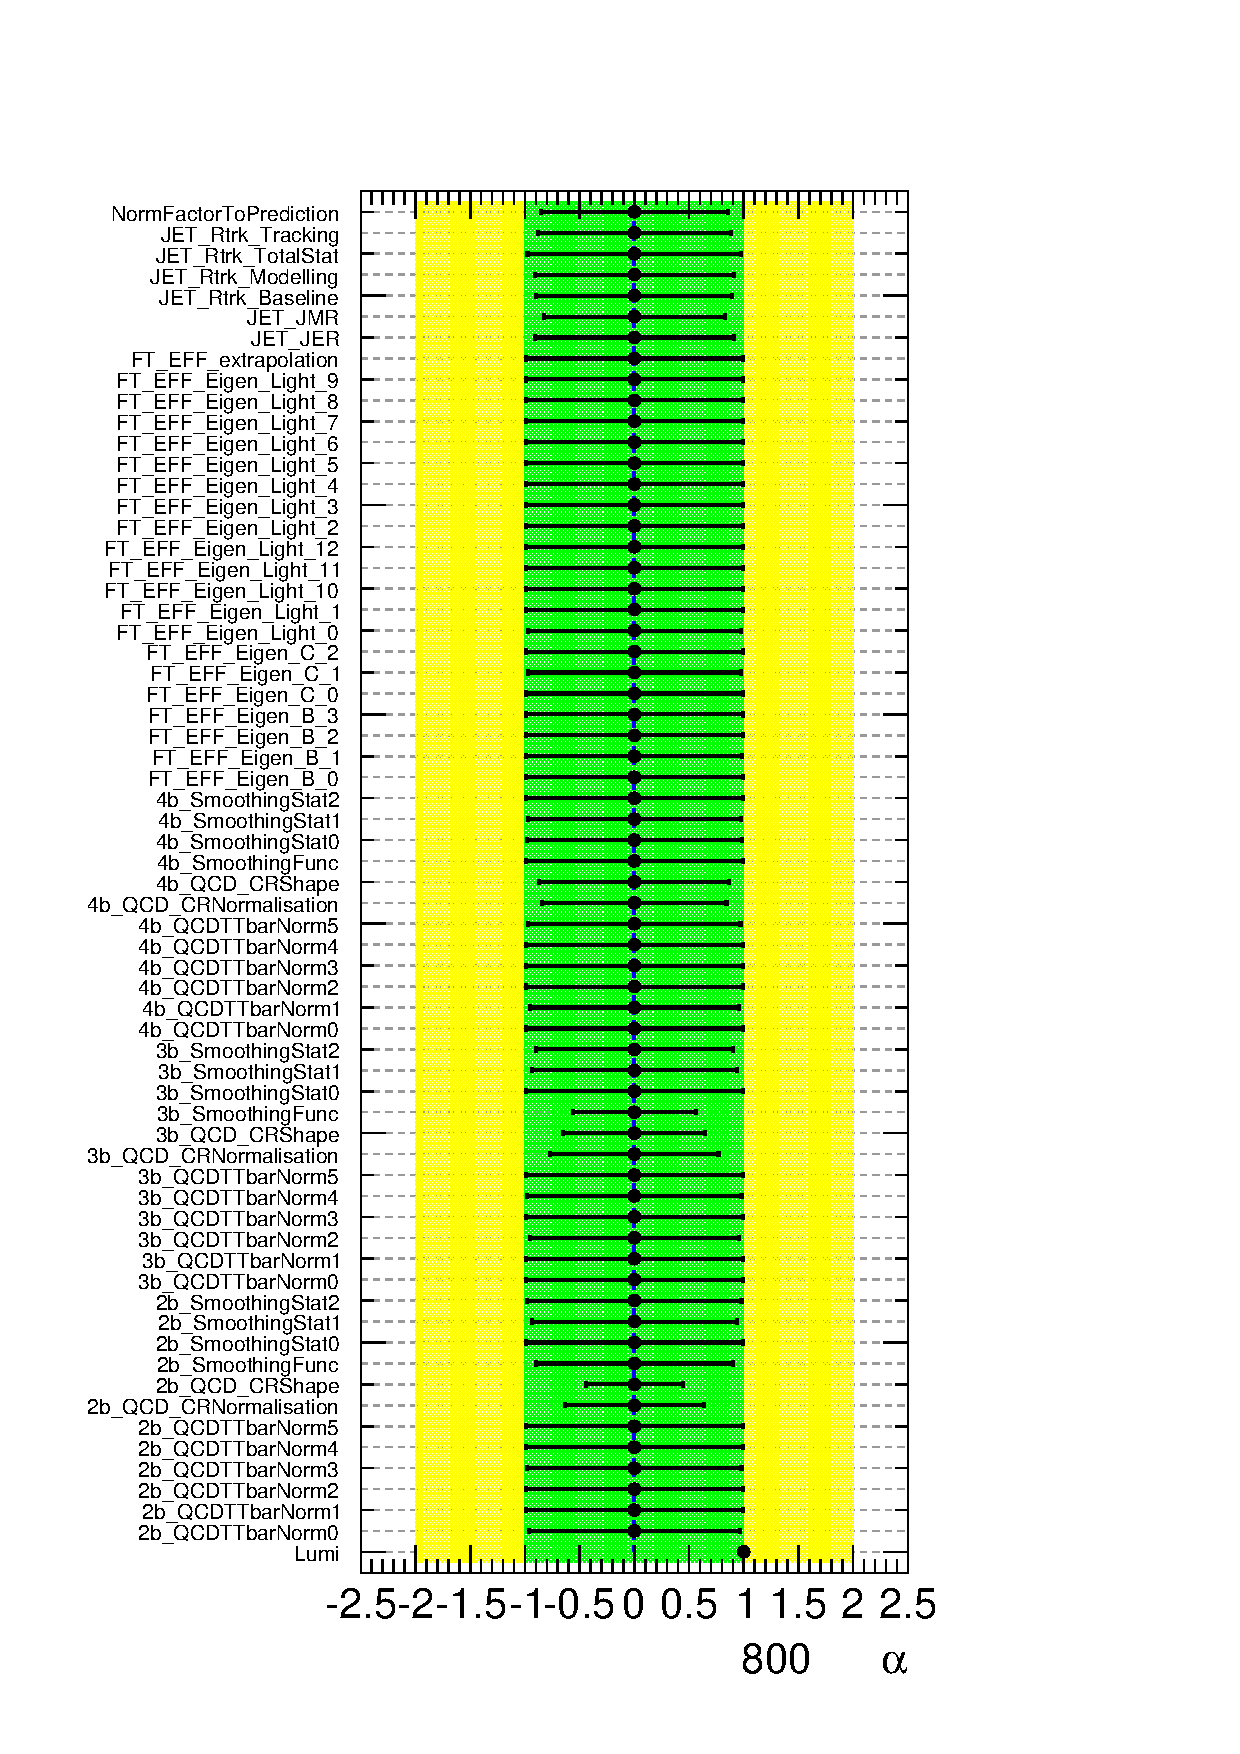
\includegraphics[angle=270, width=0.39\textwidth]{./figures/boosted/app-fitchecks/pulls_800_asimov.pdf} }
\subfloat[]{ 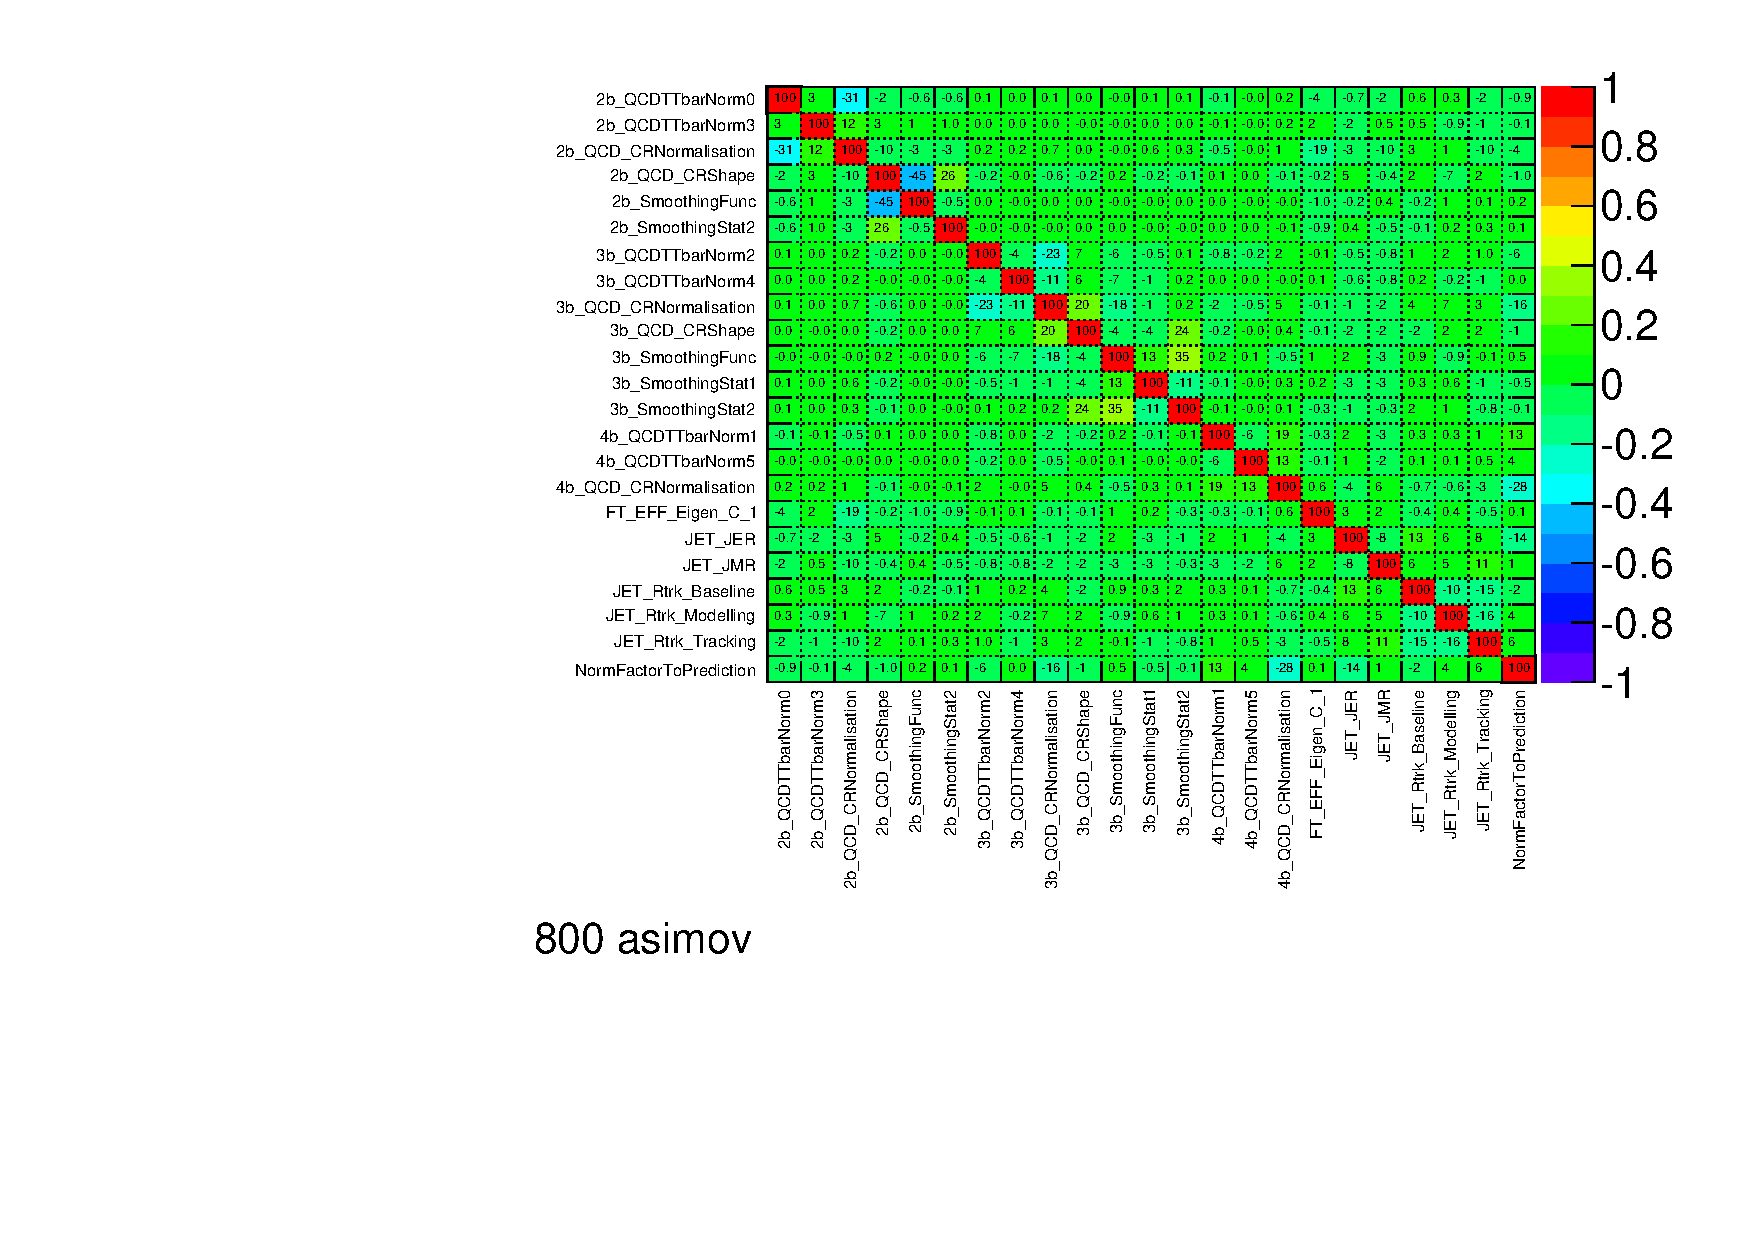
\includegraphics[angle=270, width=0.59\textwidth]{./figures/boosted/app-fitchecks/corr_800_asimov.pdf} }
\caption{Pulls (a) and correlations (b) for the 800 GeV mass point.}
\label{fig:fitchecks:pullcorr800}
\end{center}
\end{figure*}

\begin{figure*}[htbp!]
\begin{center}
\subfloat[]{ 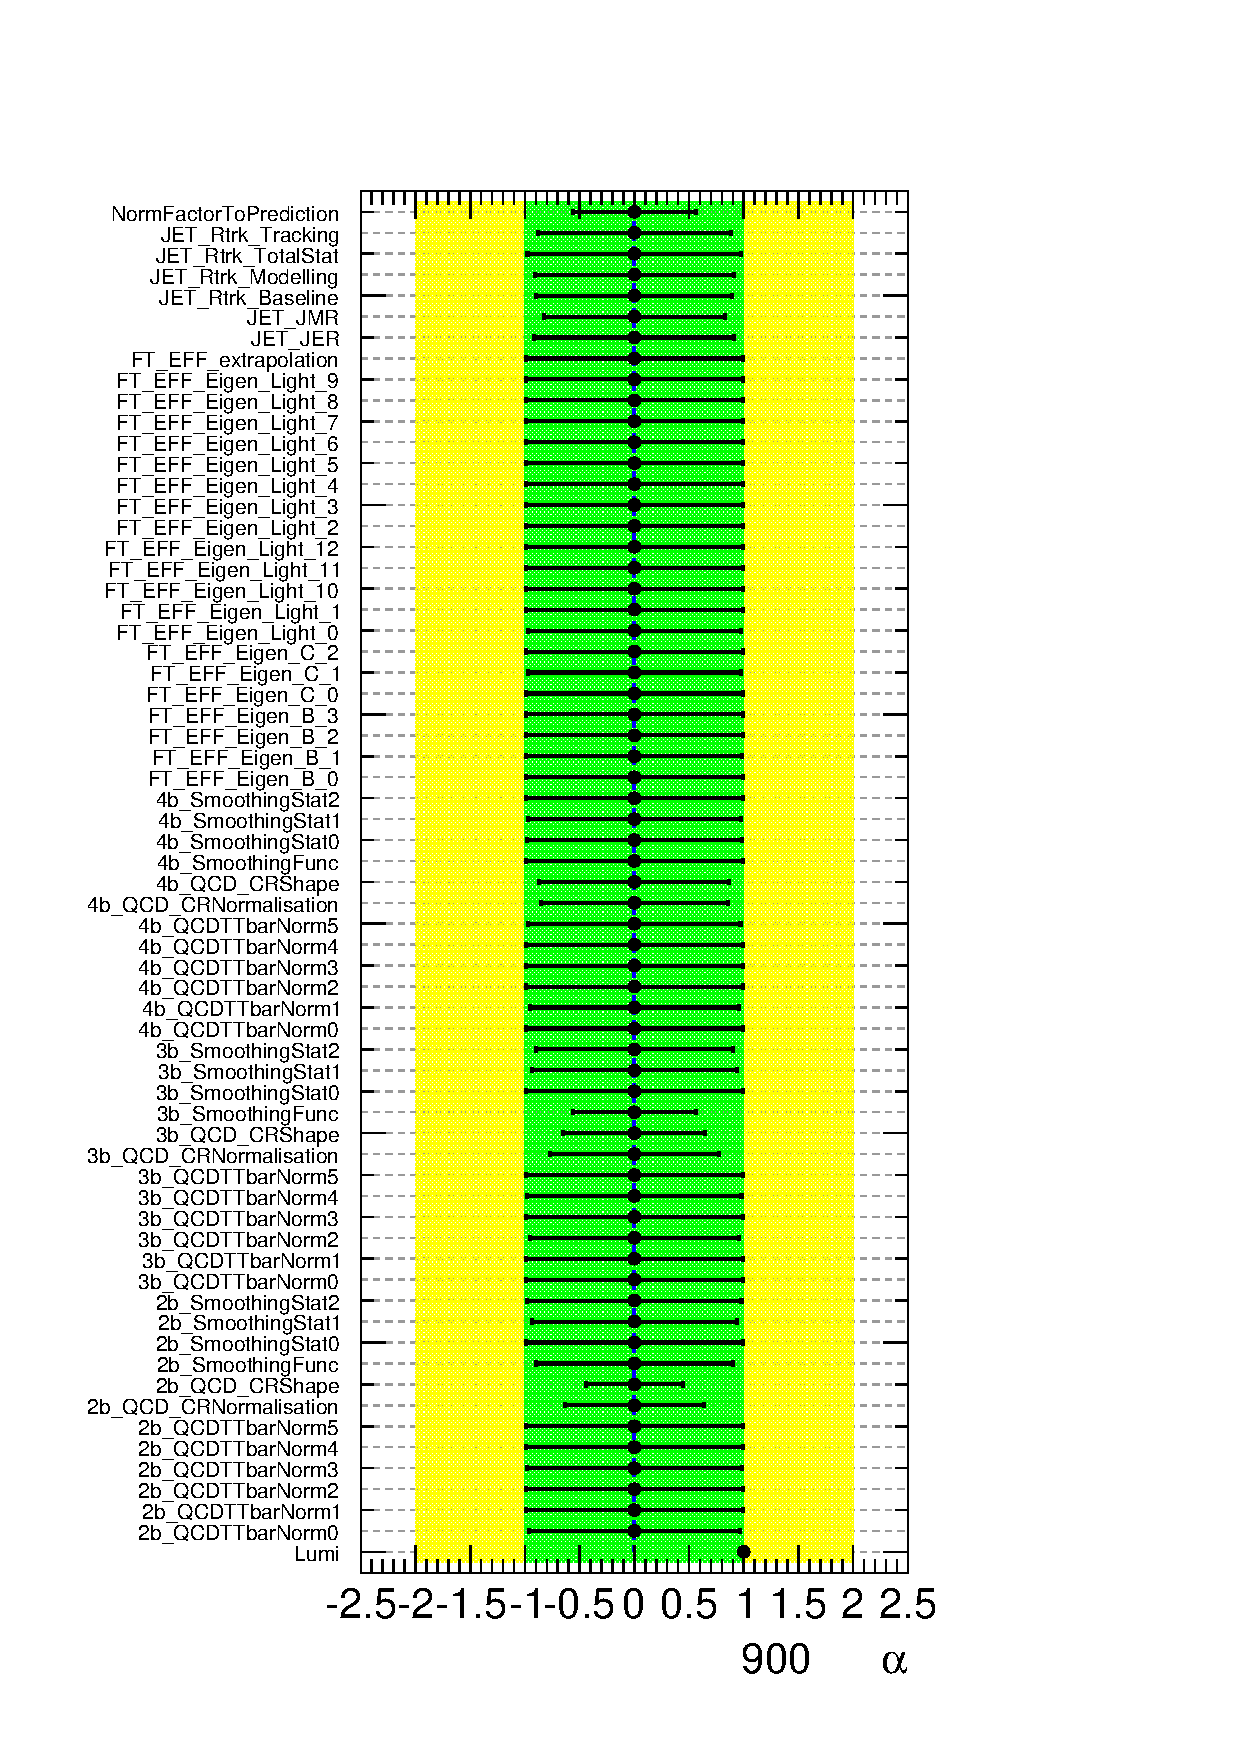
\includegraphics[angle=270, width=0.39\textwidth]{./figures/boosted/app-fitchecks/pulls_900_asimov.pdf} }
\subfloat[]{ 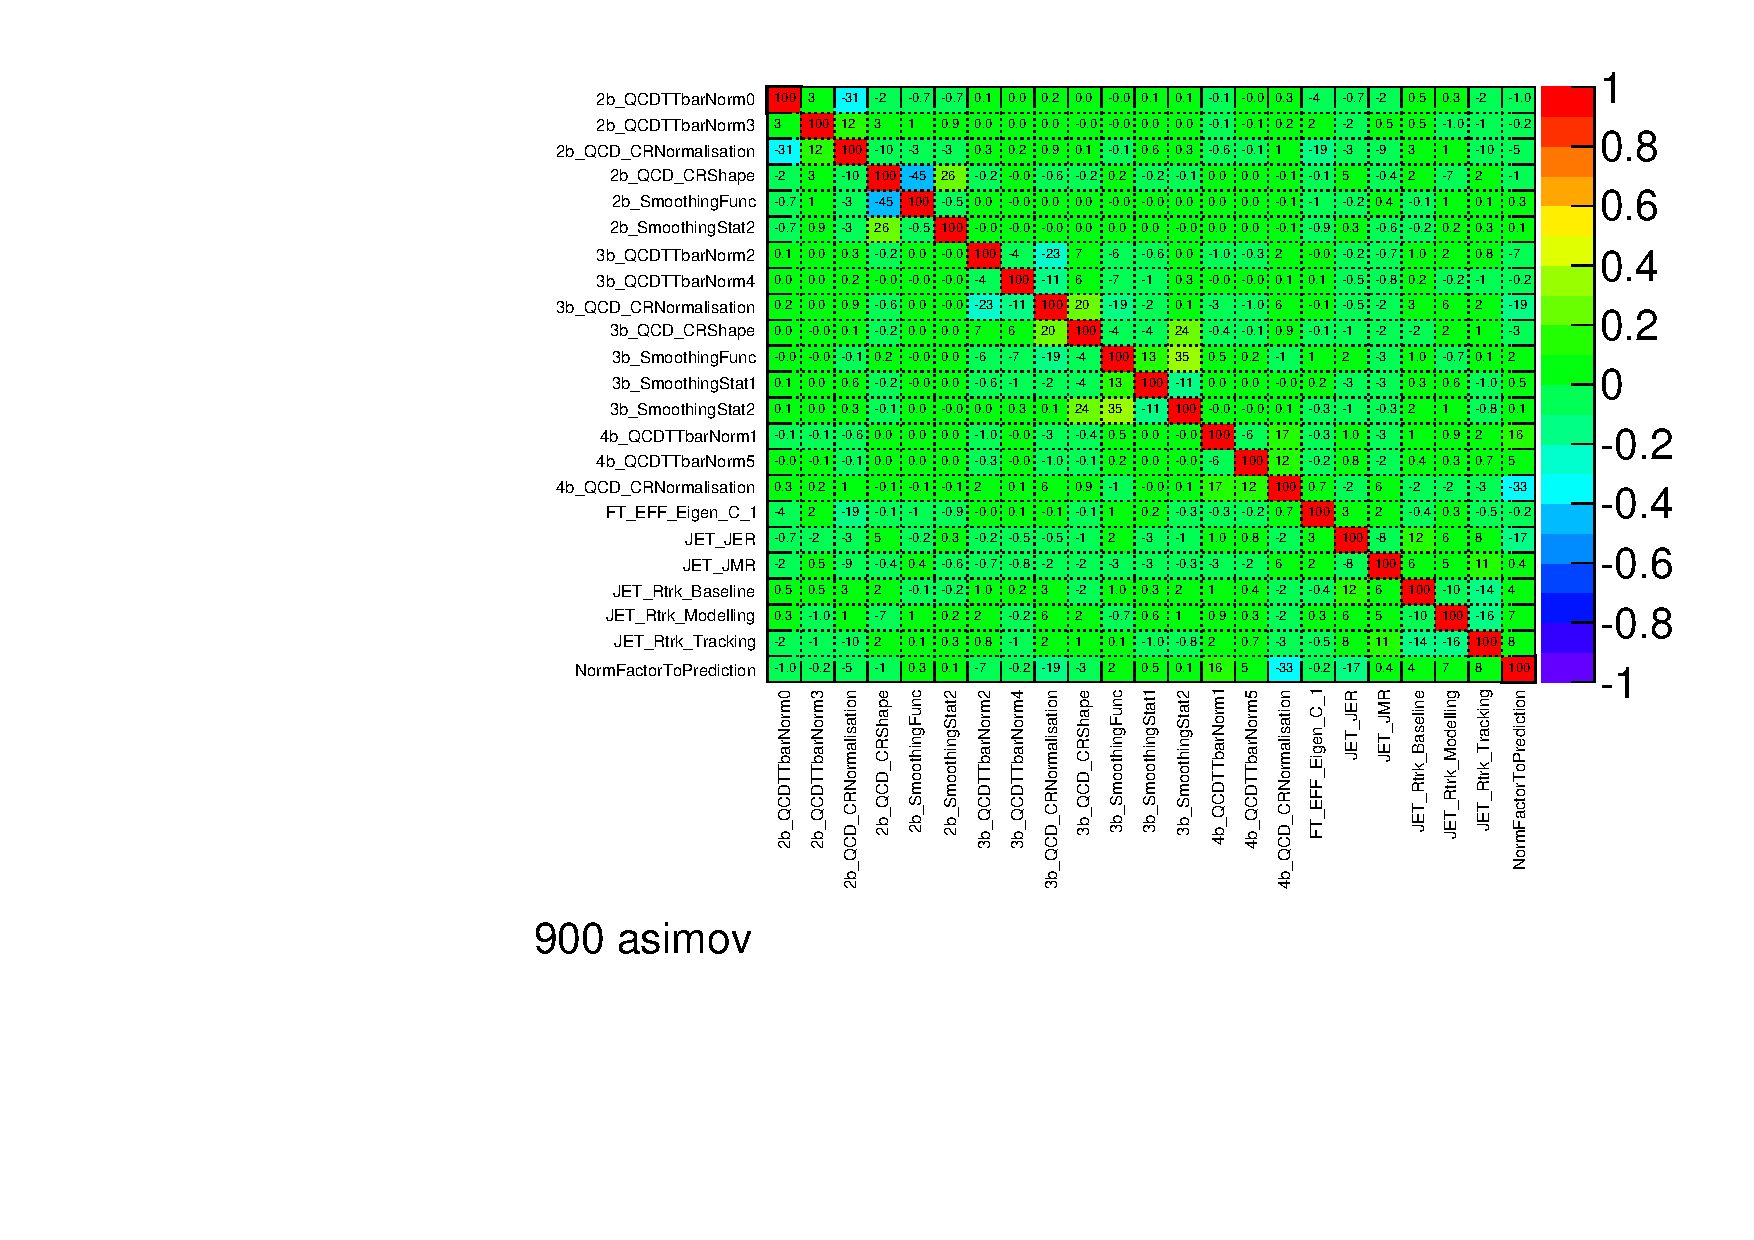
\includegraphics[angle=270, width=0.59\textwidth]{./figures/boosted/app-fitchecks/corr_900_asimov.pdf} }
\caption{Pulls (a) and correlations (b) for the 900 GeV mass point.}
\label{fig:fitchecks:pullcorr900}
\end{center}
\end{figure*}

\begin{figure*}[htbp!]
\begin{center}
\subfloat[]{ 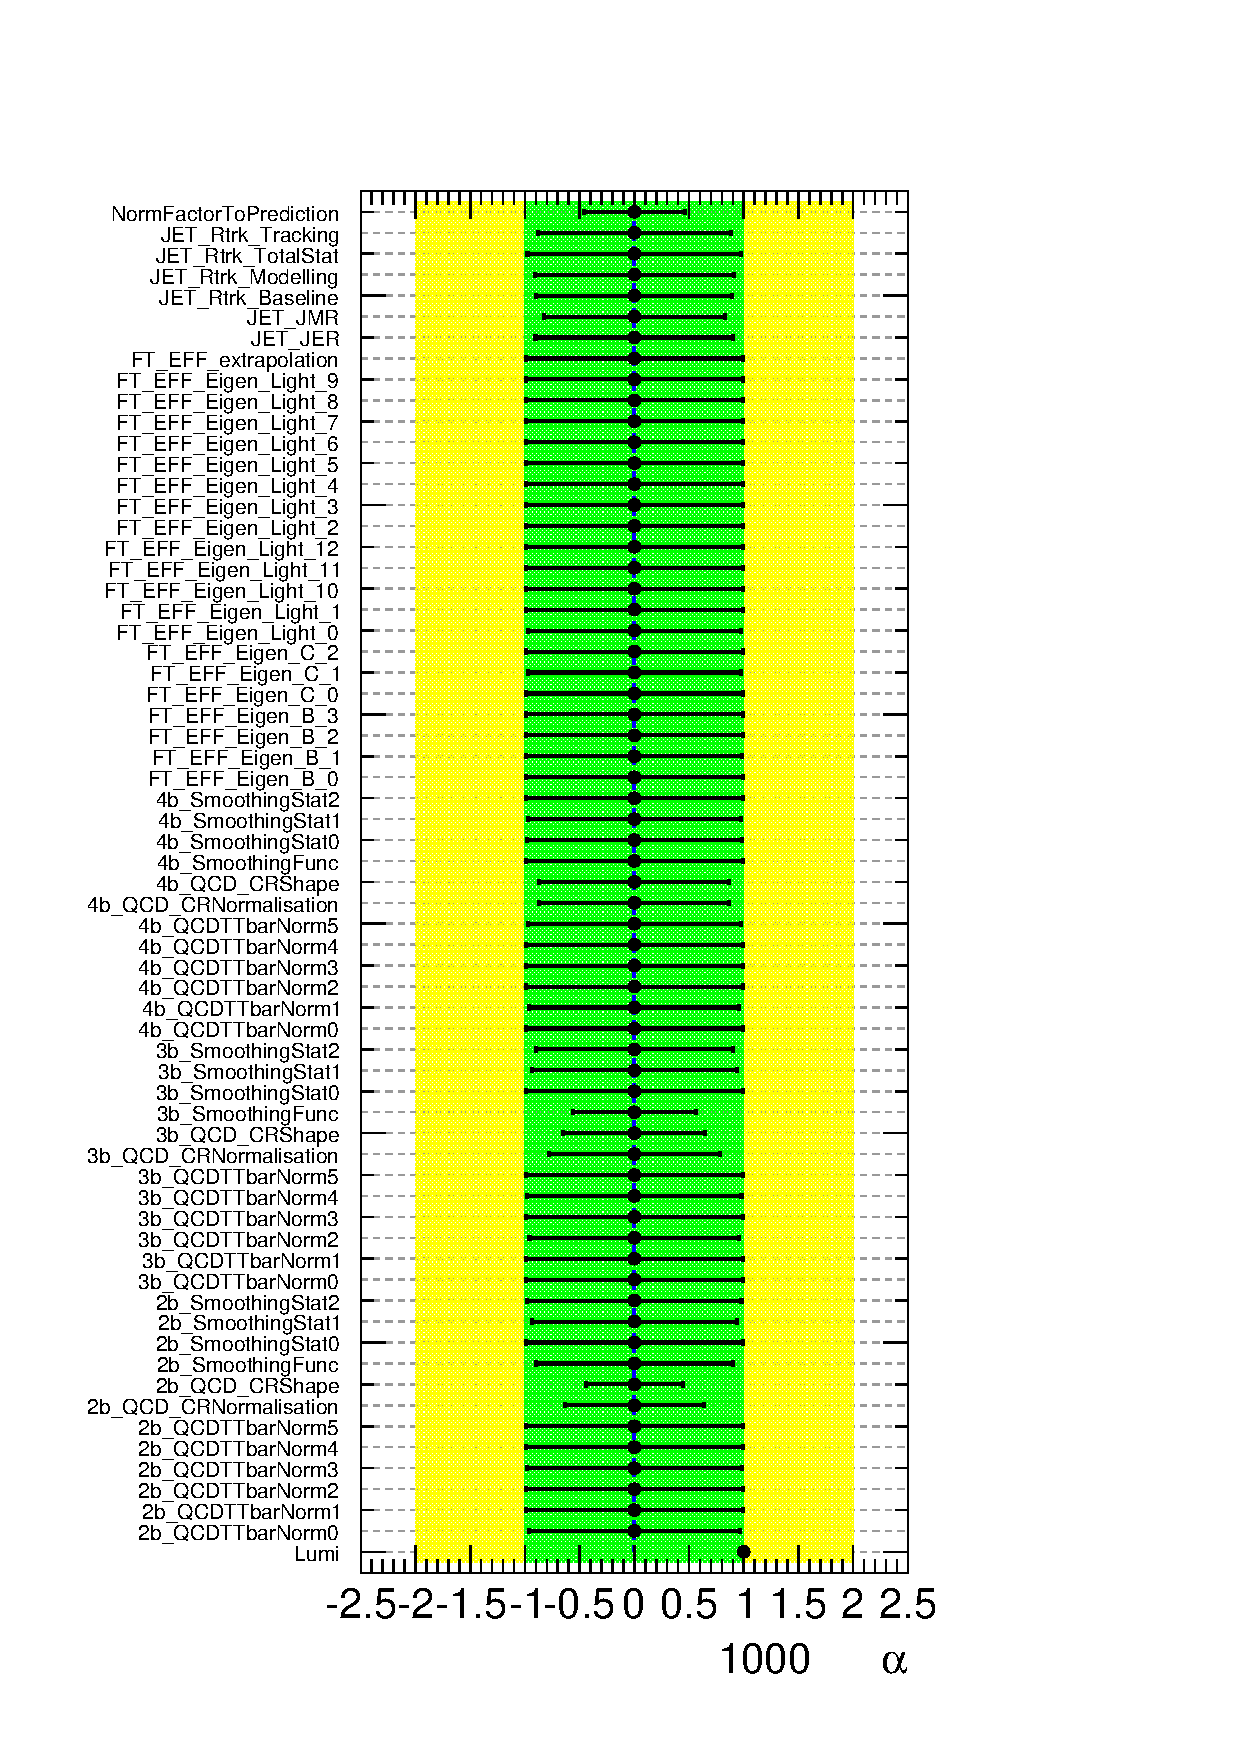
\includegraphics[angle=270, width=0.39\textwidth]{./figures/boosted/app-fitchecks/pulls_1000_asimov.pdf} }
\subfloat[]{ 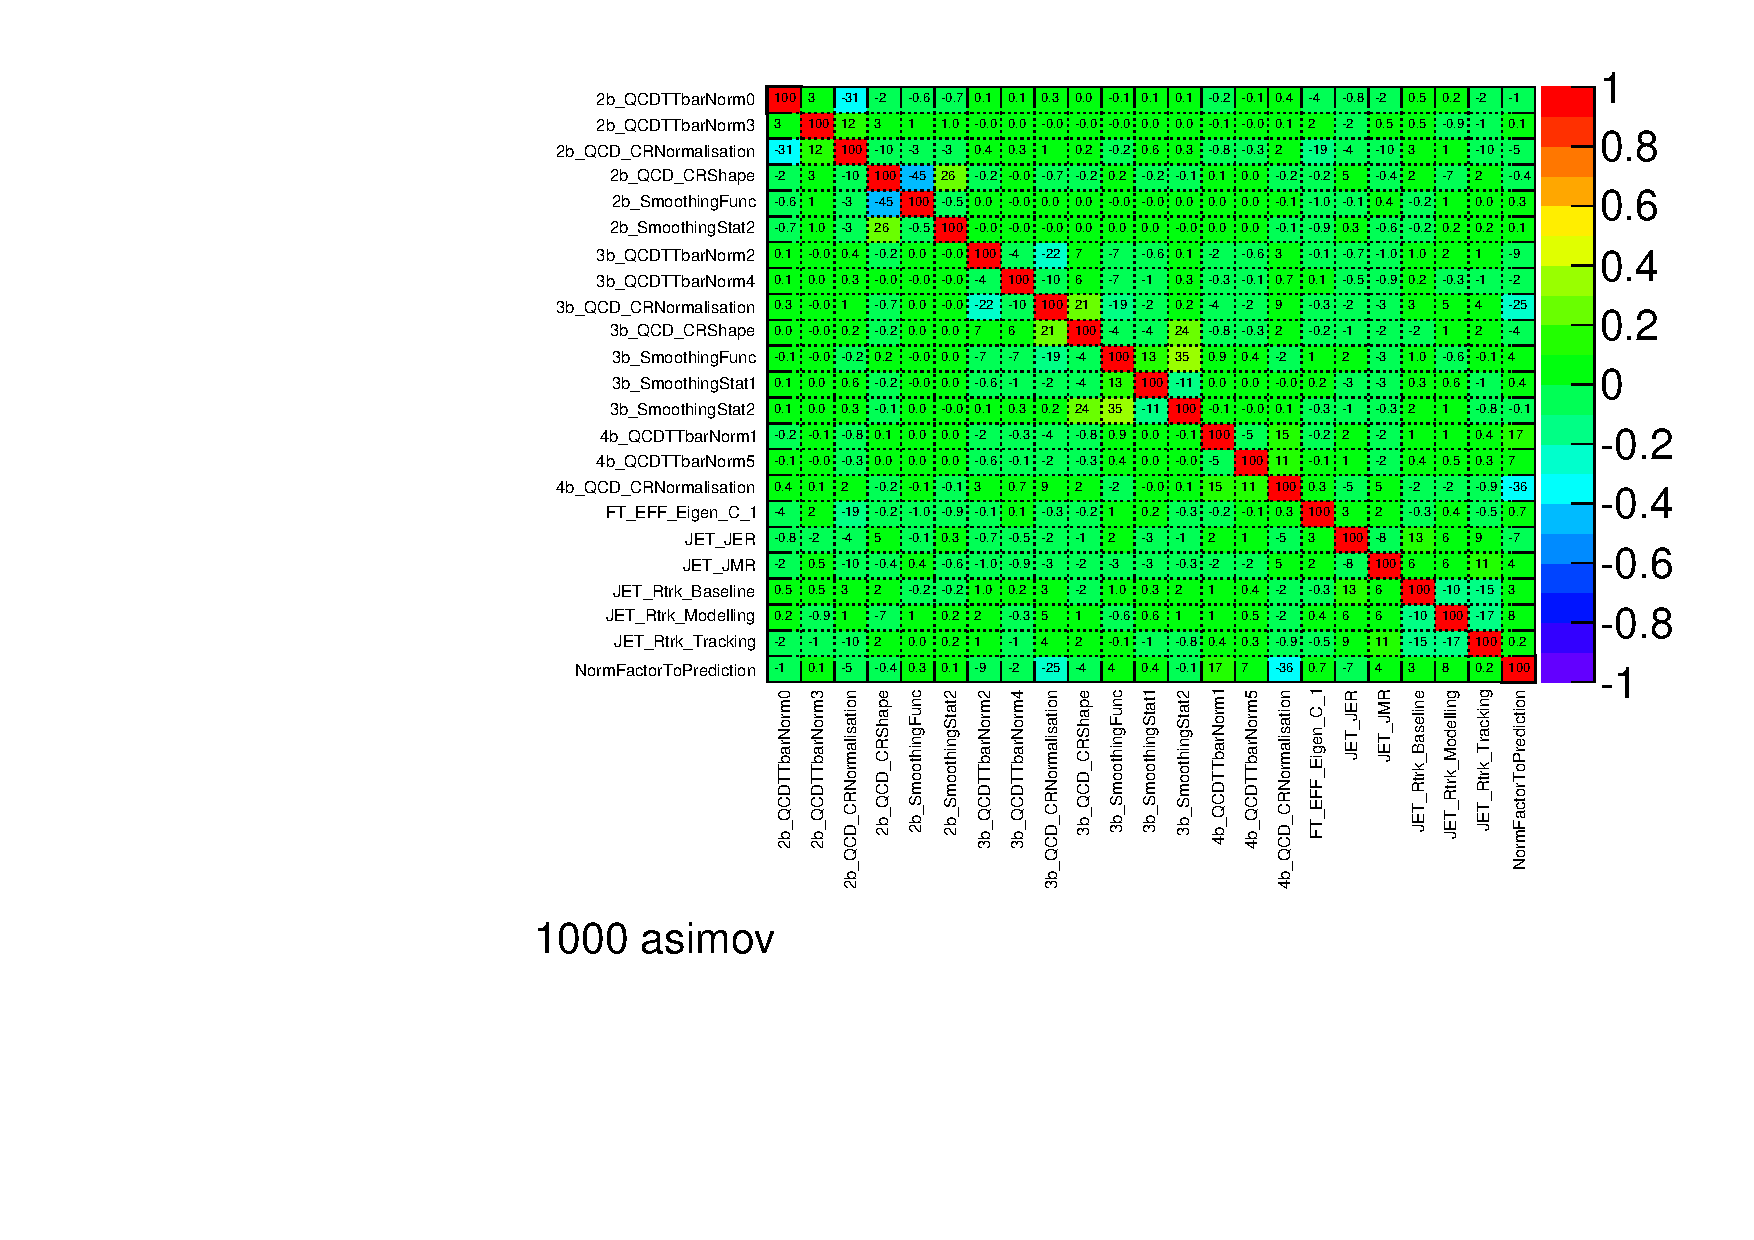
\includegraphics[angle=270, width=0.59\textwidth]{./figures/boosted/app-fitchecks/corr_1000_asimov.pdf} }
\caption{Pulls (a) and correlations (b) for the 1000 GeV mass point.}
\label{fig:fitchecks:pullcorr1000}
\end{center}
\end{figure*}

\begin{figure*}[htbp!]
\begin{center}
\subfloat[]{ 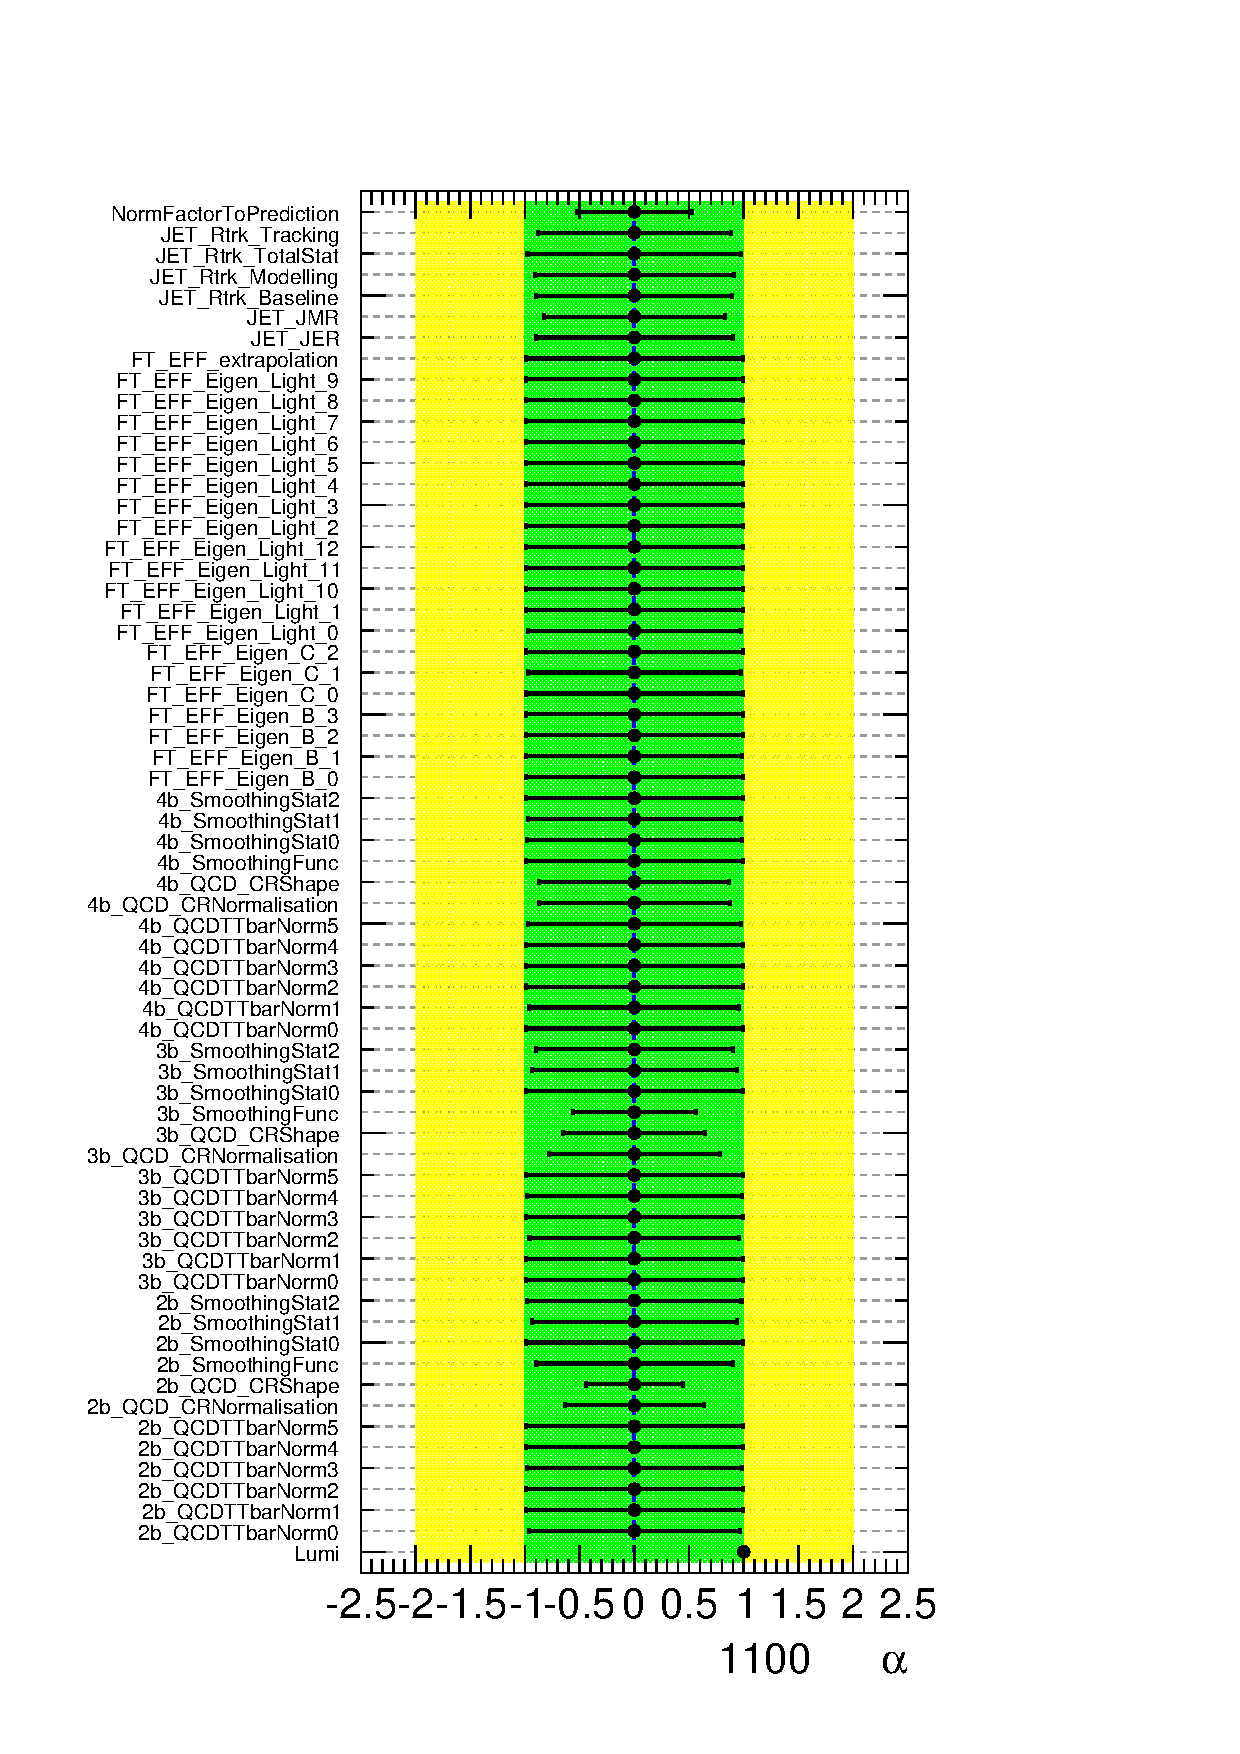
\includegraphics[angle=270, width=0.39\textwidth]{./figures/boosted/app-fitchecks/pulls_1100_asimov.pdf} }
\subfloat[]{ 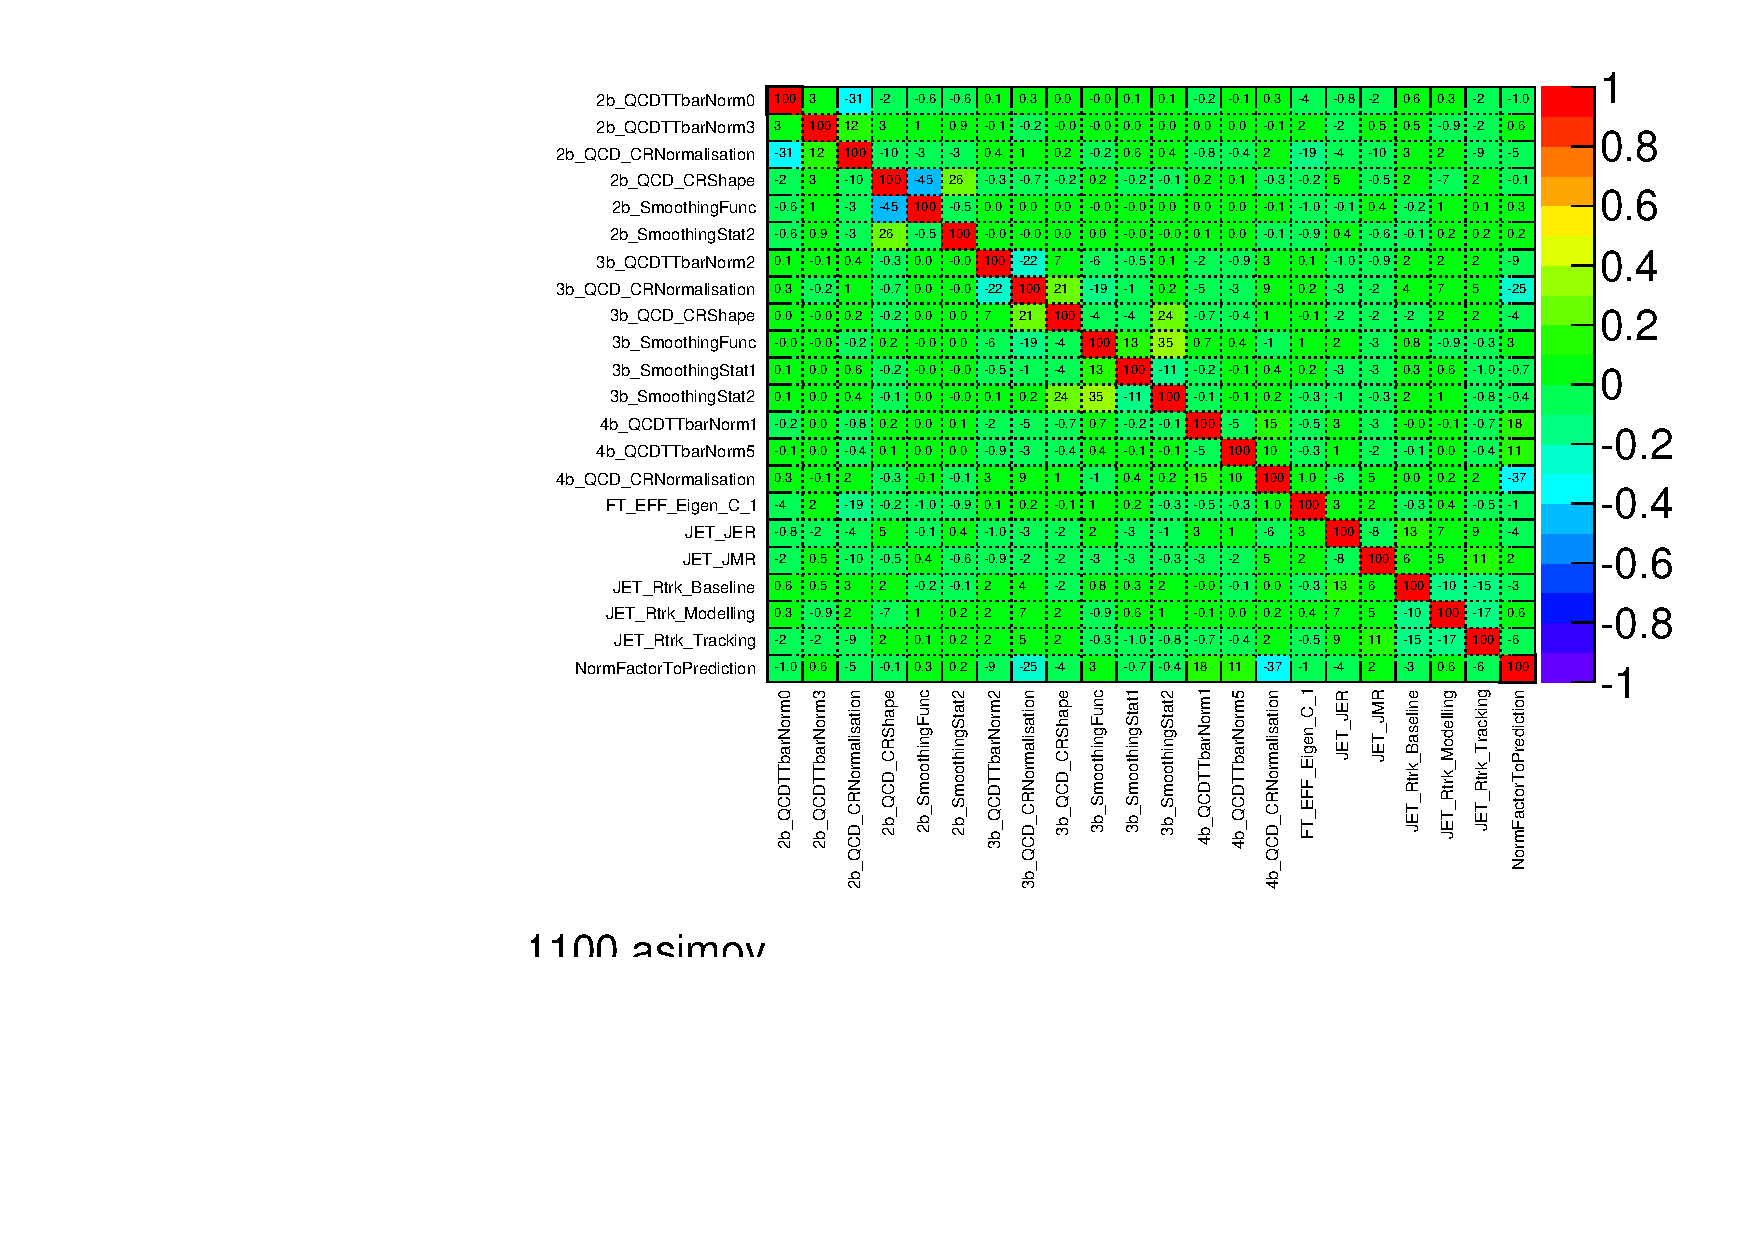
\includegraphics[angle=270, width=0.59\textwidth]{./figures/boosted/app-fitchecks/corr_1100_asimov.pdf} }
\caption{Pulls (a) and correlations (b) for the 1100 GeV mass point.}
\label{fig:fitchecks:pullcorr1100}
\end{center}
\end{figure*}

\begin{figure*}[htbp!]
\begin{center}
\subfloat[]{ 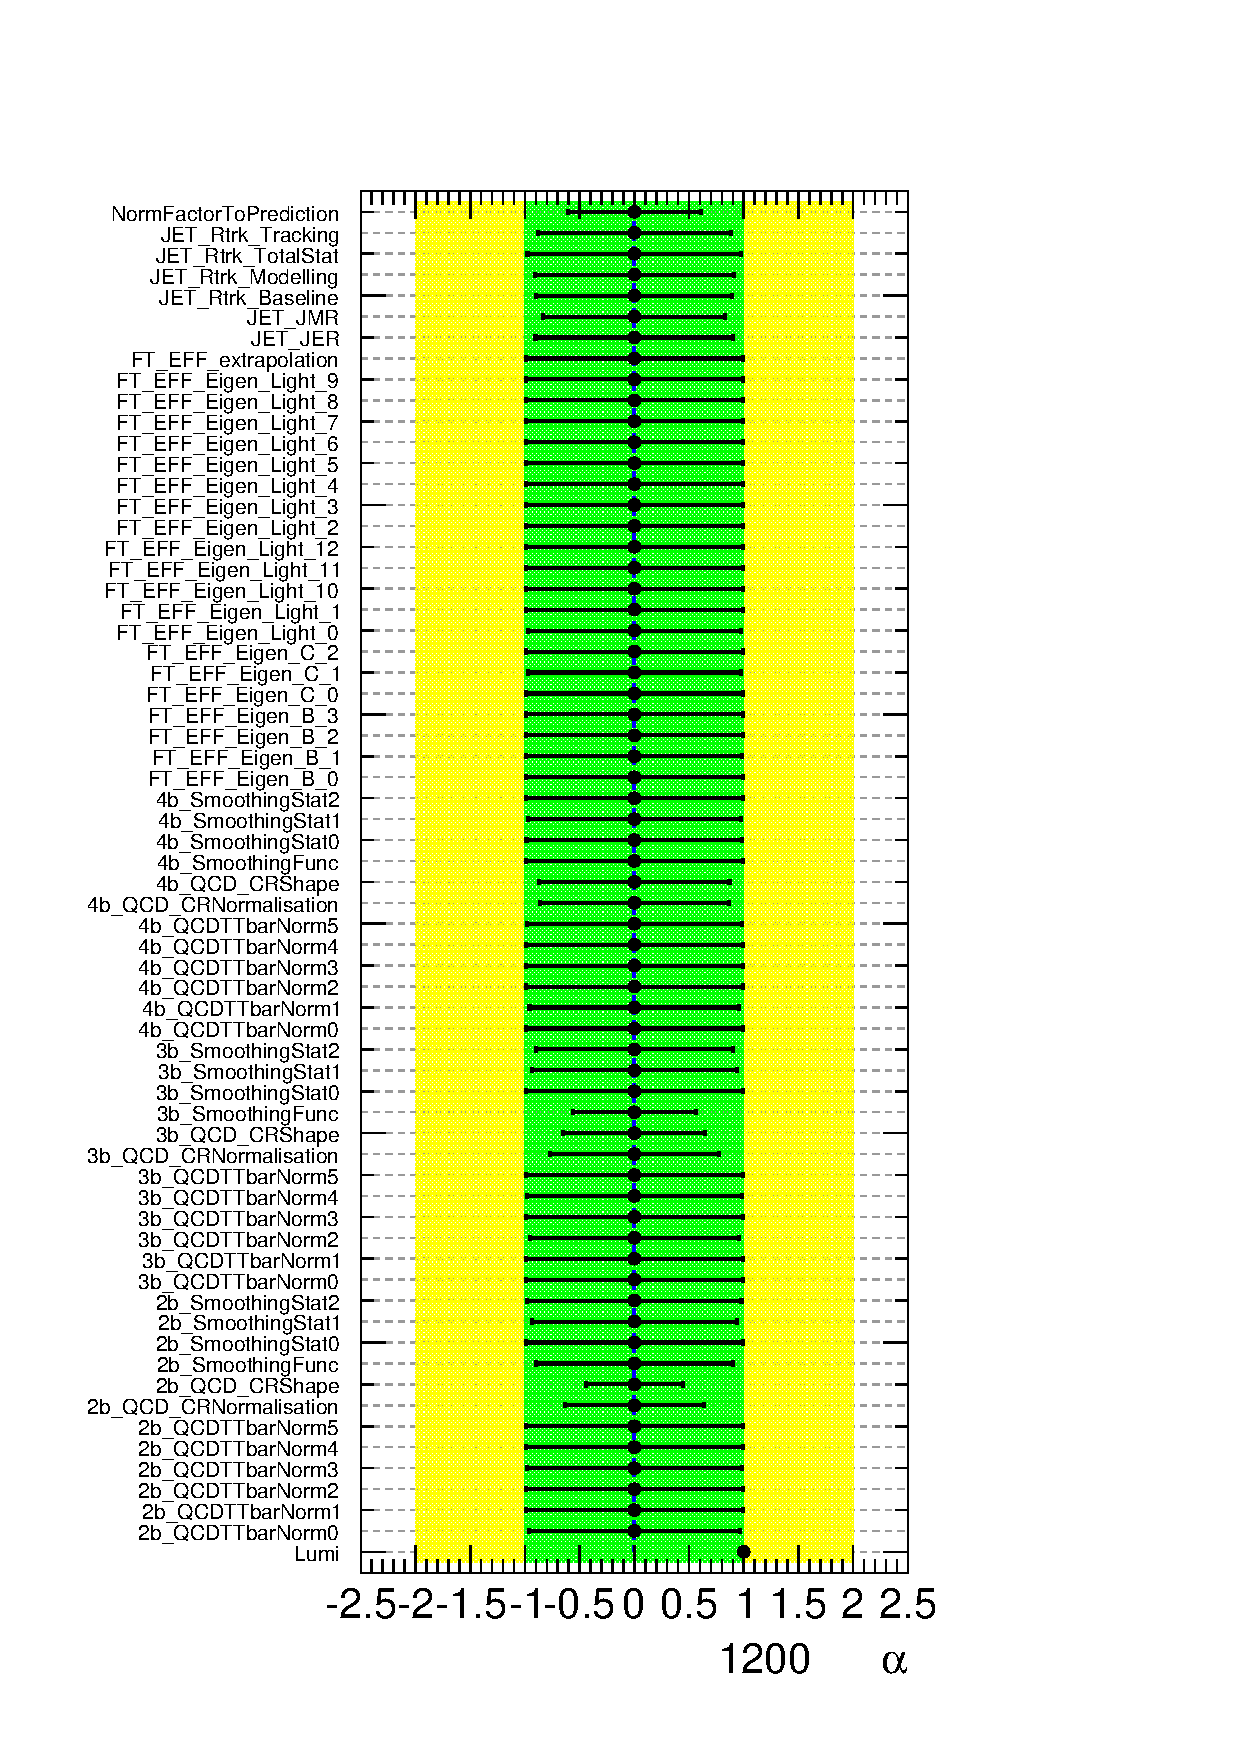
\includegraphics[angle=270, width=0.39\textwidth]{./figures/boosted/app-fitchecks/pulls_1200_asimov.pdf} }
\subfloat[]{ 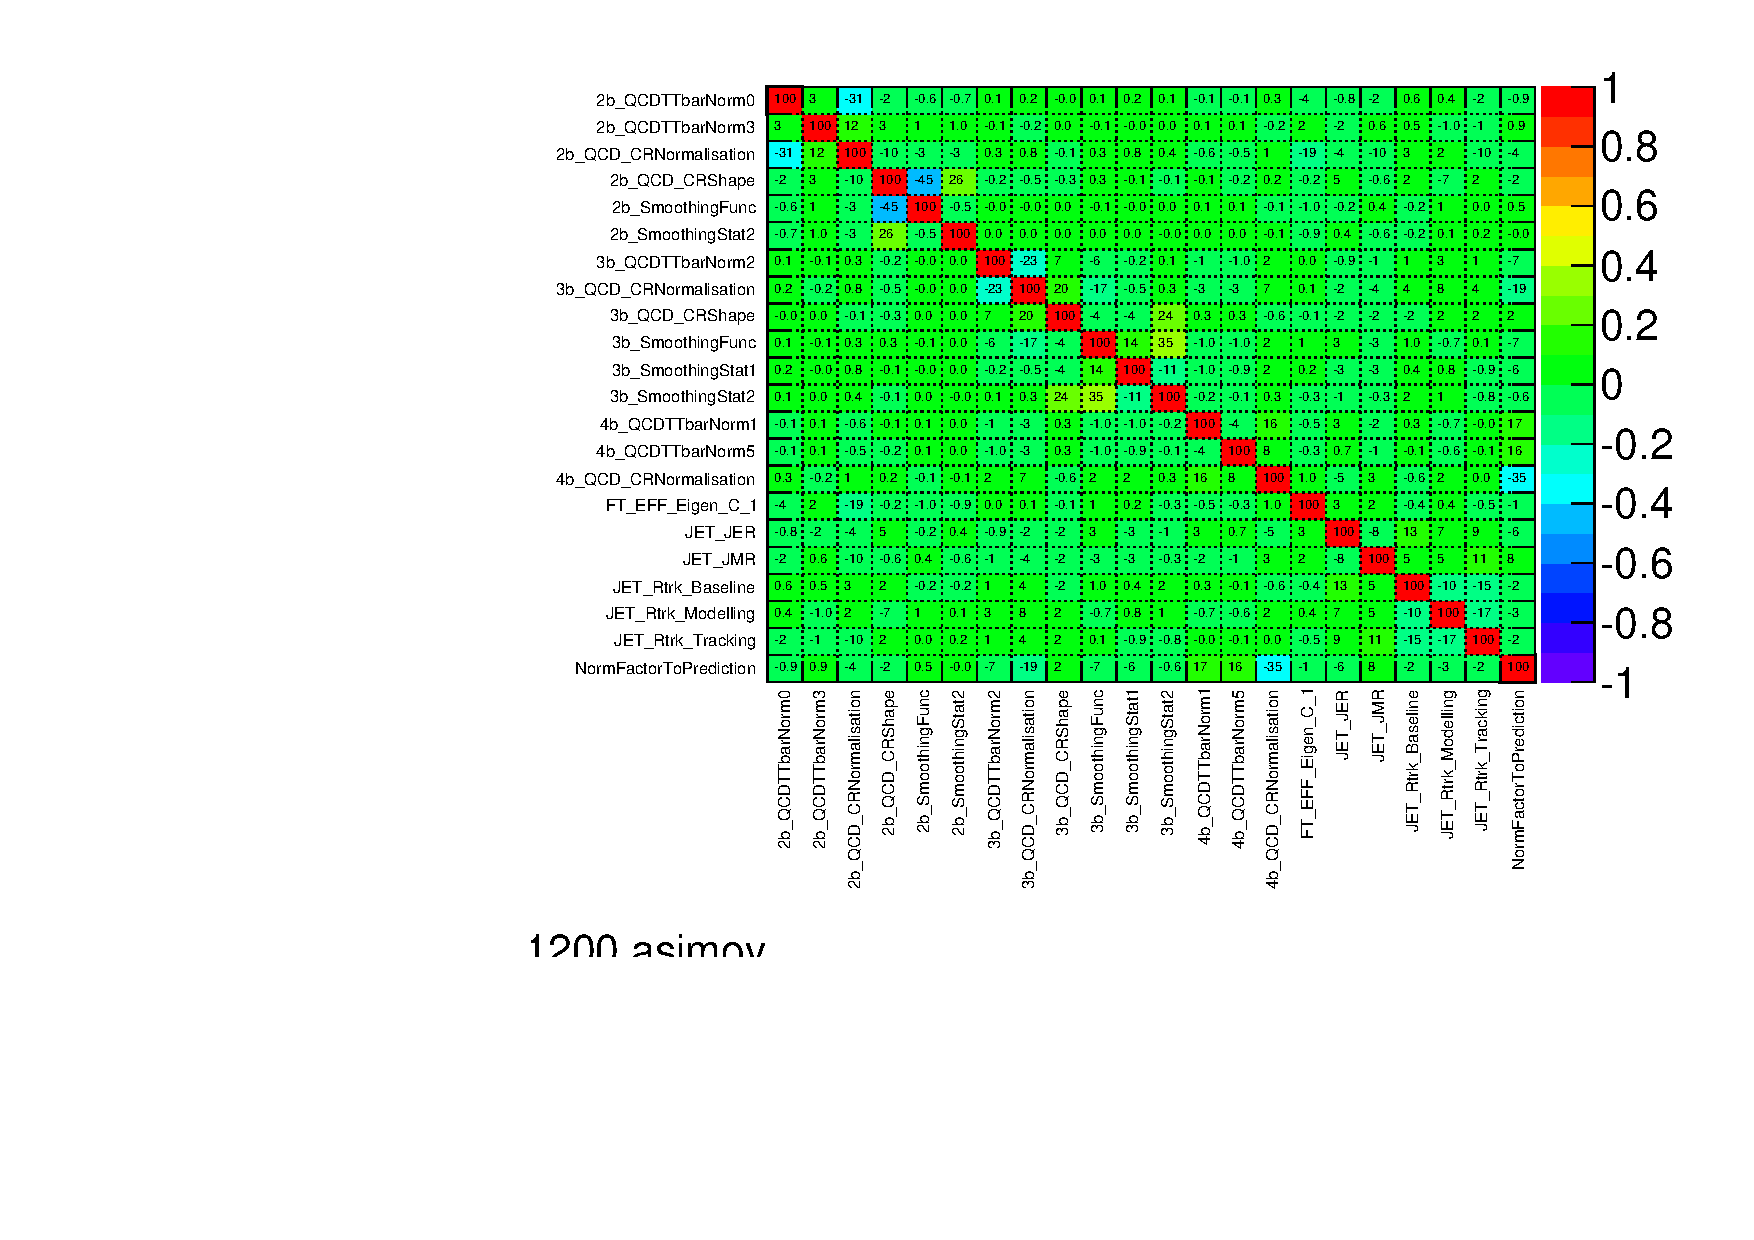
\includegraphics[angle=270, width=0.59\textwidth]{./figures/boosted/app-fitchecks/corr_1200_asimov.pdf} }
\caption{Pulls (a) and correlations (b) for the 1200 GeV mass point.}
\label{fig:fitchecks:pullcorr1200}
\end{center}
\end{figure*}

\begin{figure*}[htbp!]
\begin{center}
\subfloat[]{ 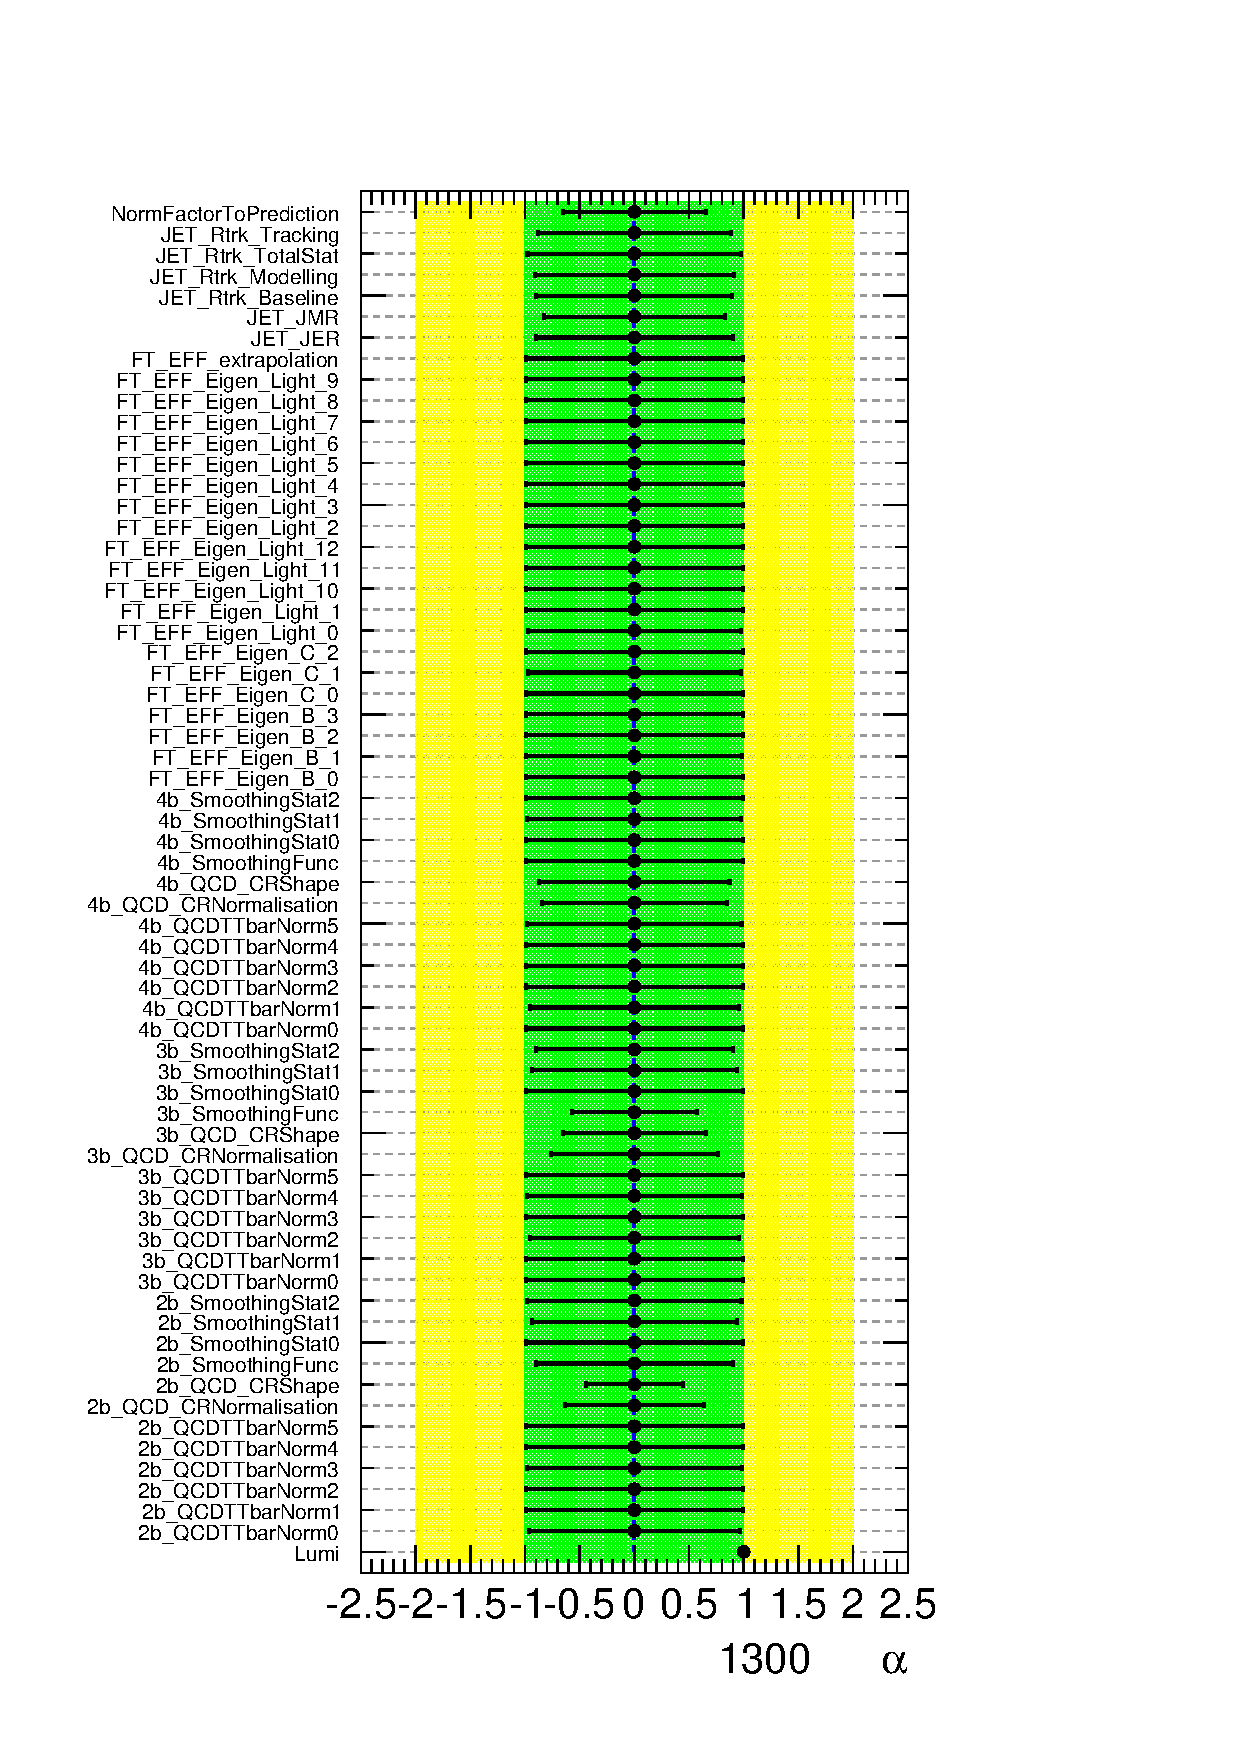
\includegraphics[angle=270, width=0.39\textwidth]{./figures/boosted/app-fitchecks/pulls_1300_asimov.pdf} }
\subfloat[]{ 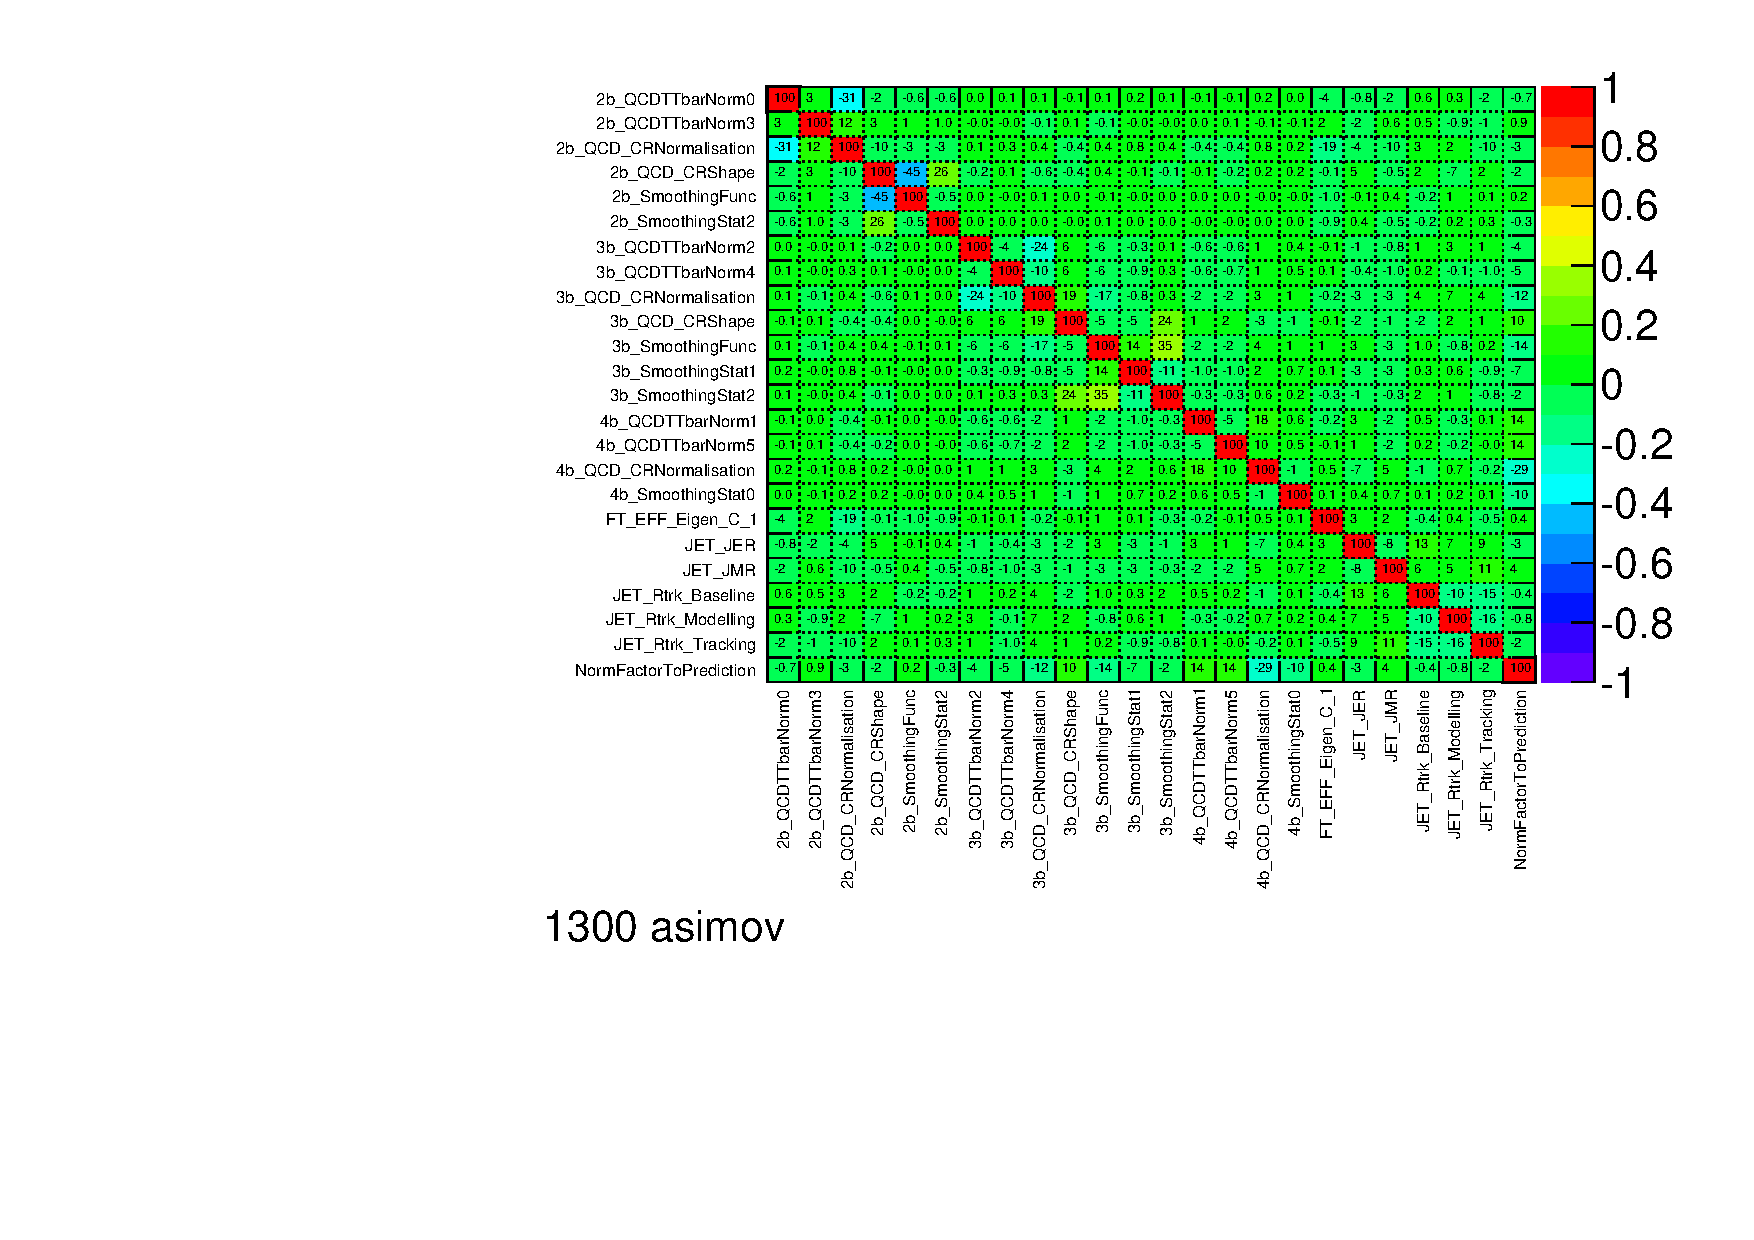
\includegraphics[angle=270, width=0.59\textwidth]{./figures/boosted/app-fitchecks/corr_1300_asimov.pdf} }
\caption{Pulls (a) and correlations (b) for the 1300 GeV mass point.}
\label{fig:fitchecks:pullcorr1300}
\end{center}
\end{figure*}

\begin{figure*}[htbp!]
\begin{center}
\subfloat[]{ 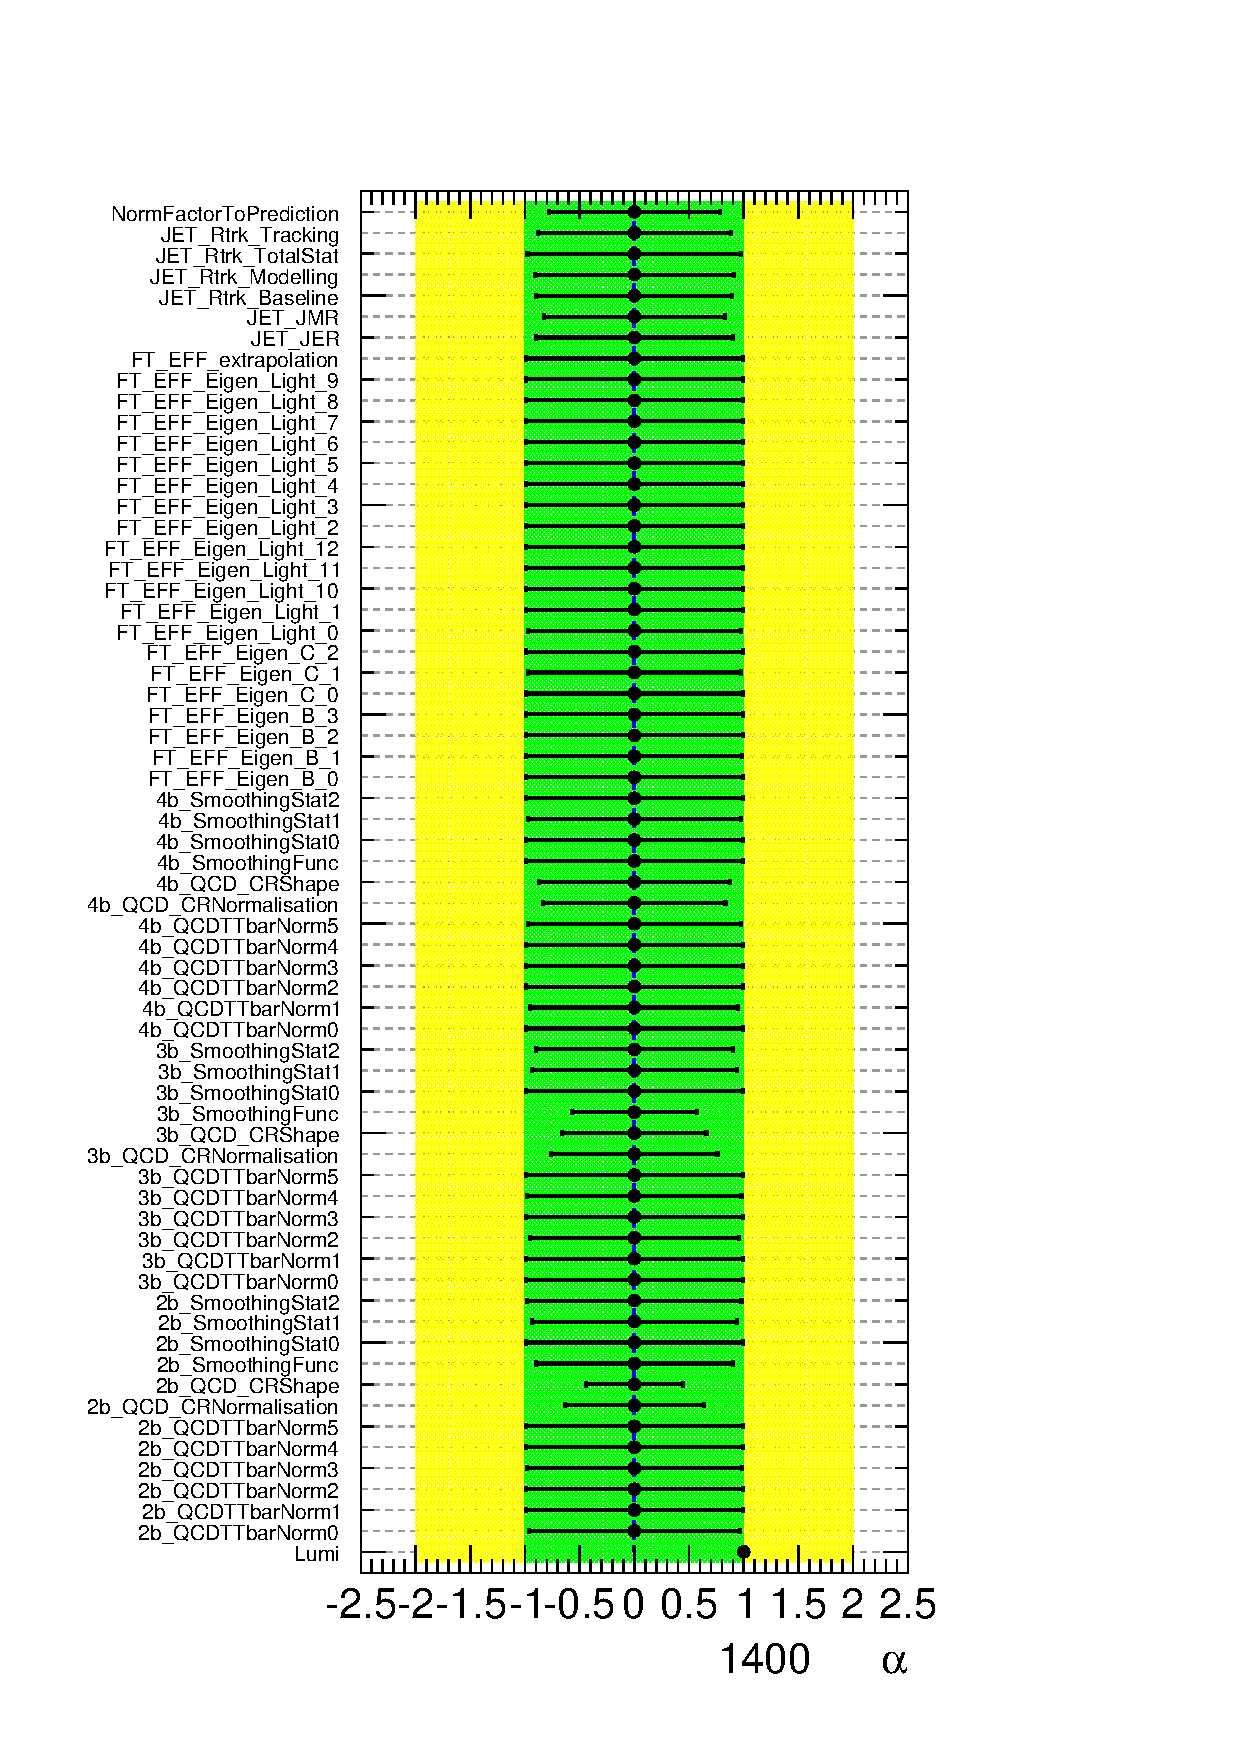
\includegraphics[angle=270, width=0.39\textwidth]{./figures/boosted/app-fitchecks/pulls_1400_asimov.pdf} }
\subfloat[]{ 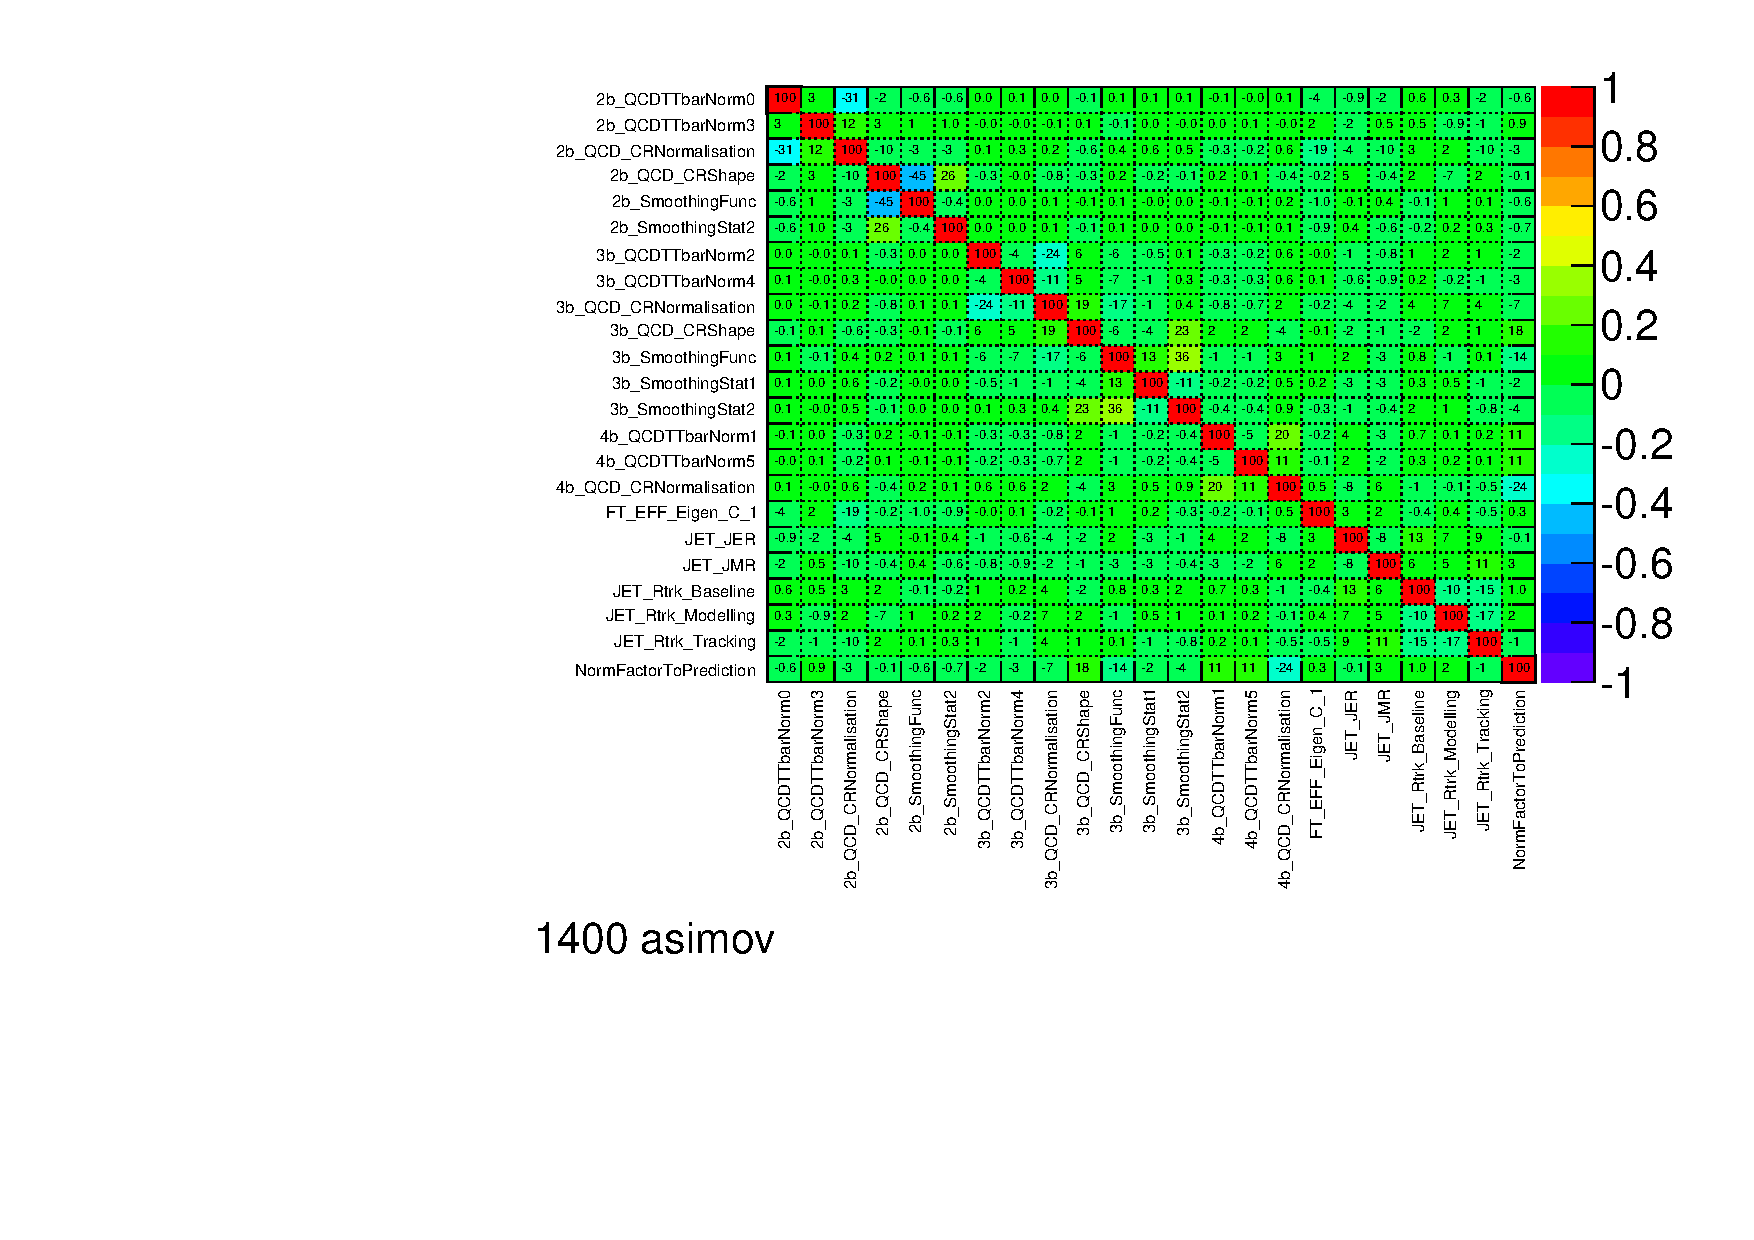
\includegraphics[angle=270, width=0.59\textwidth]{./figures/boosted/app-fitchecks/corr_1400_asimov.pdf} }
\caption{Pulls (a) and correlations (b) for the 1400 GeV mass point.}
\label{fig:fitchecks:pullcorr1400}
\end{center}
\end{figure*}

\begin{figure*}[htbp!]
\begin{center}
\subfloat[]{ 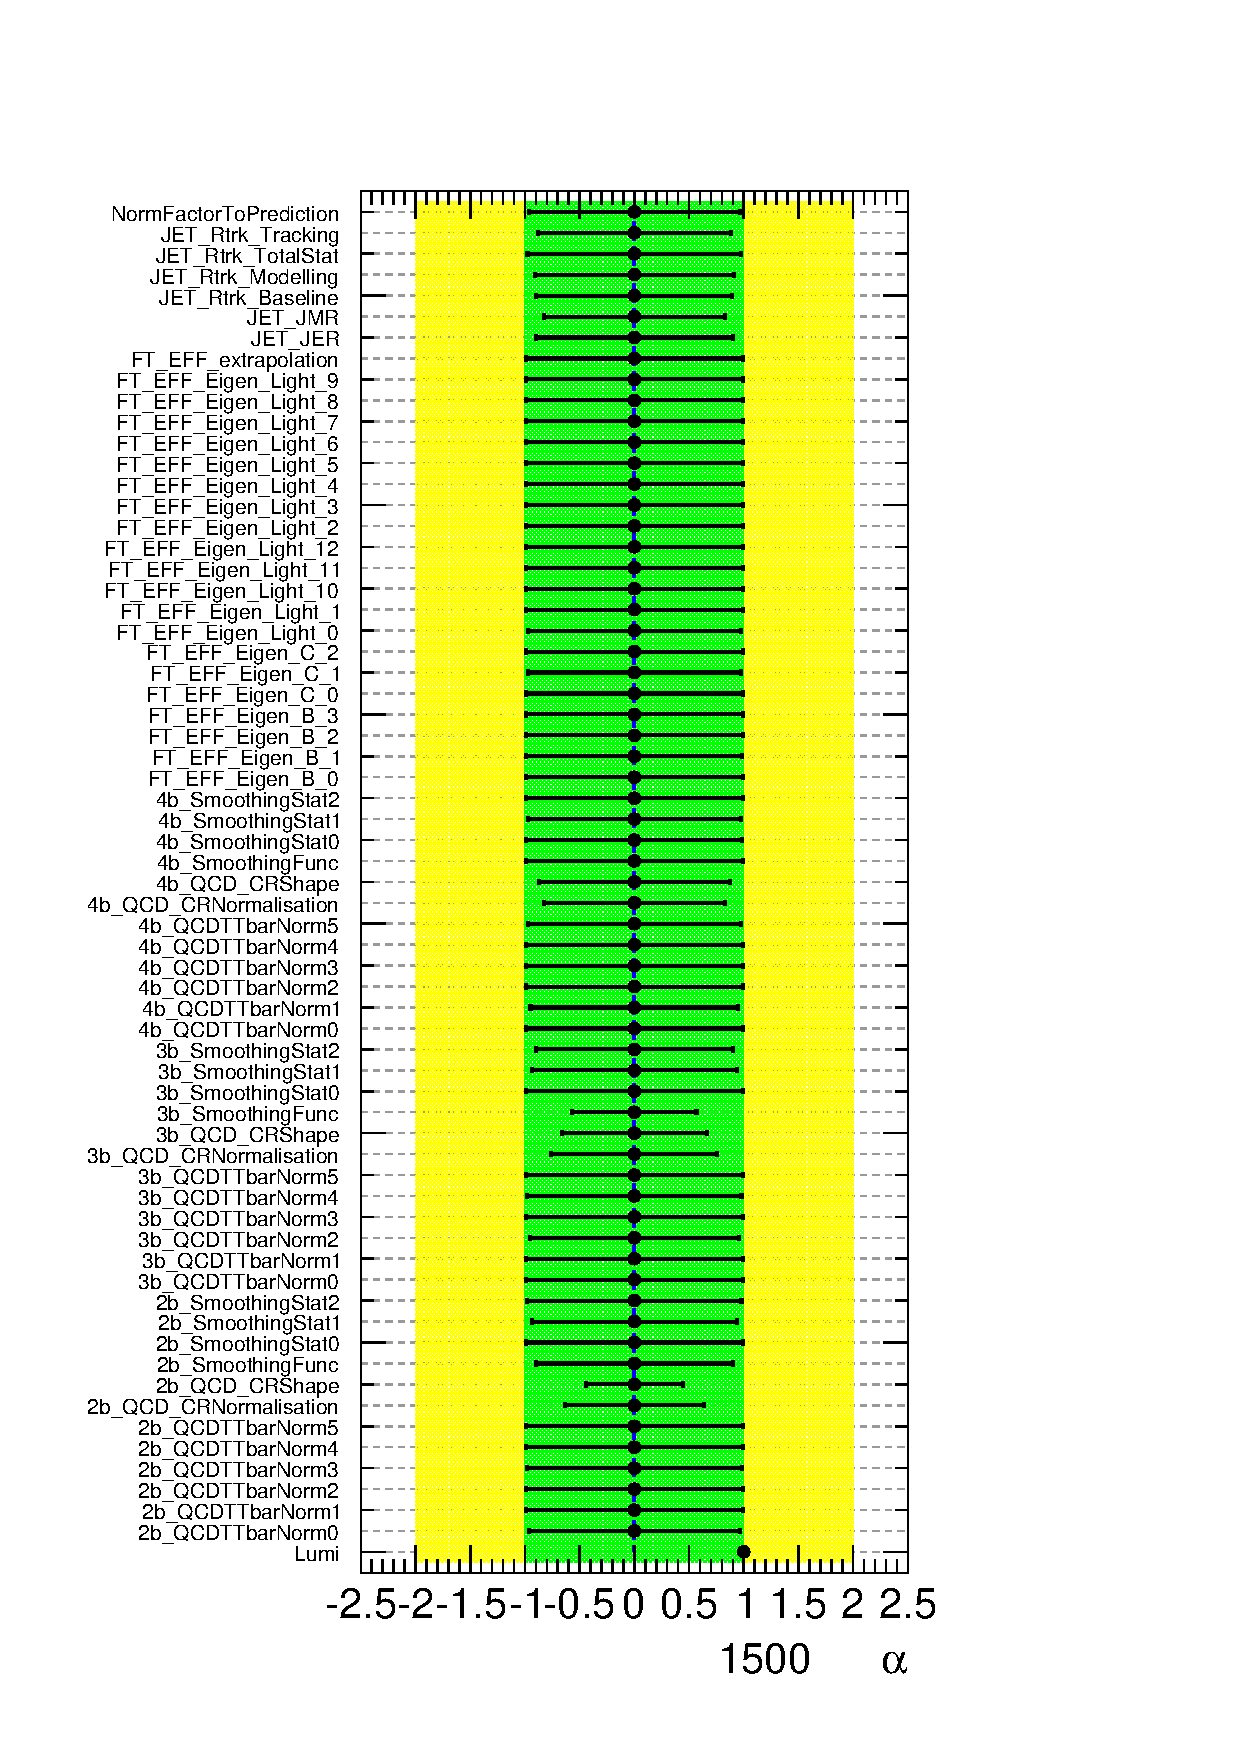
\includegraphics[angle=270, width=0.39\textwidth]{./figures/boosted/app-fitchecks/pulls_1500_asimov.pdf} }
\subfloat[]{ 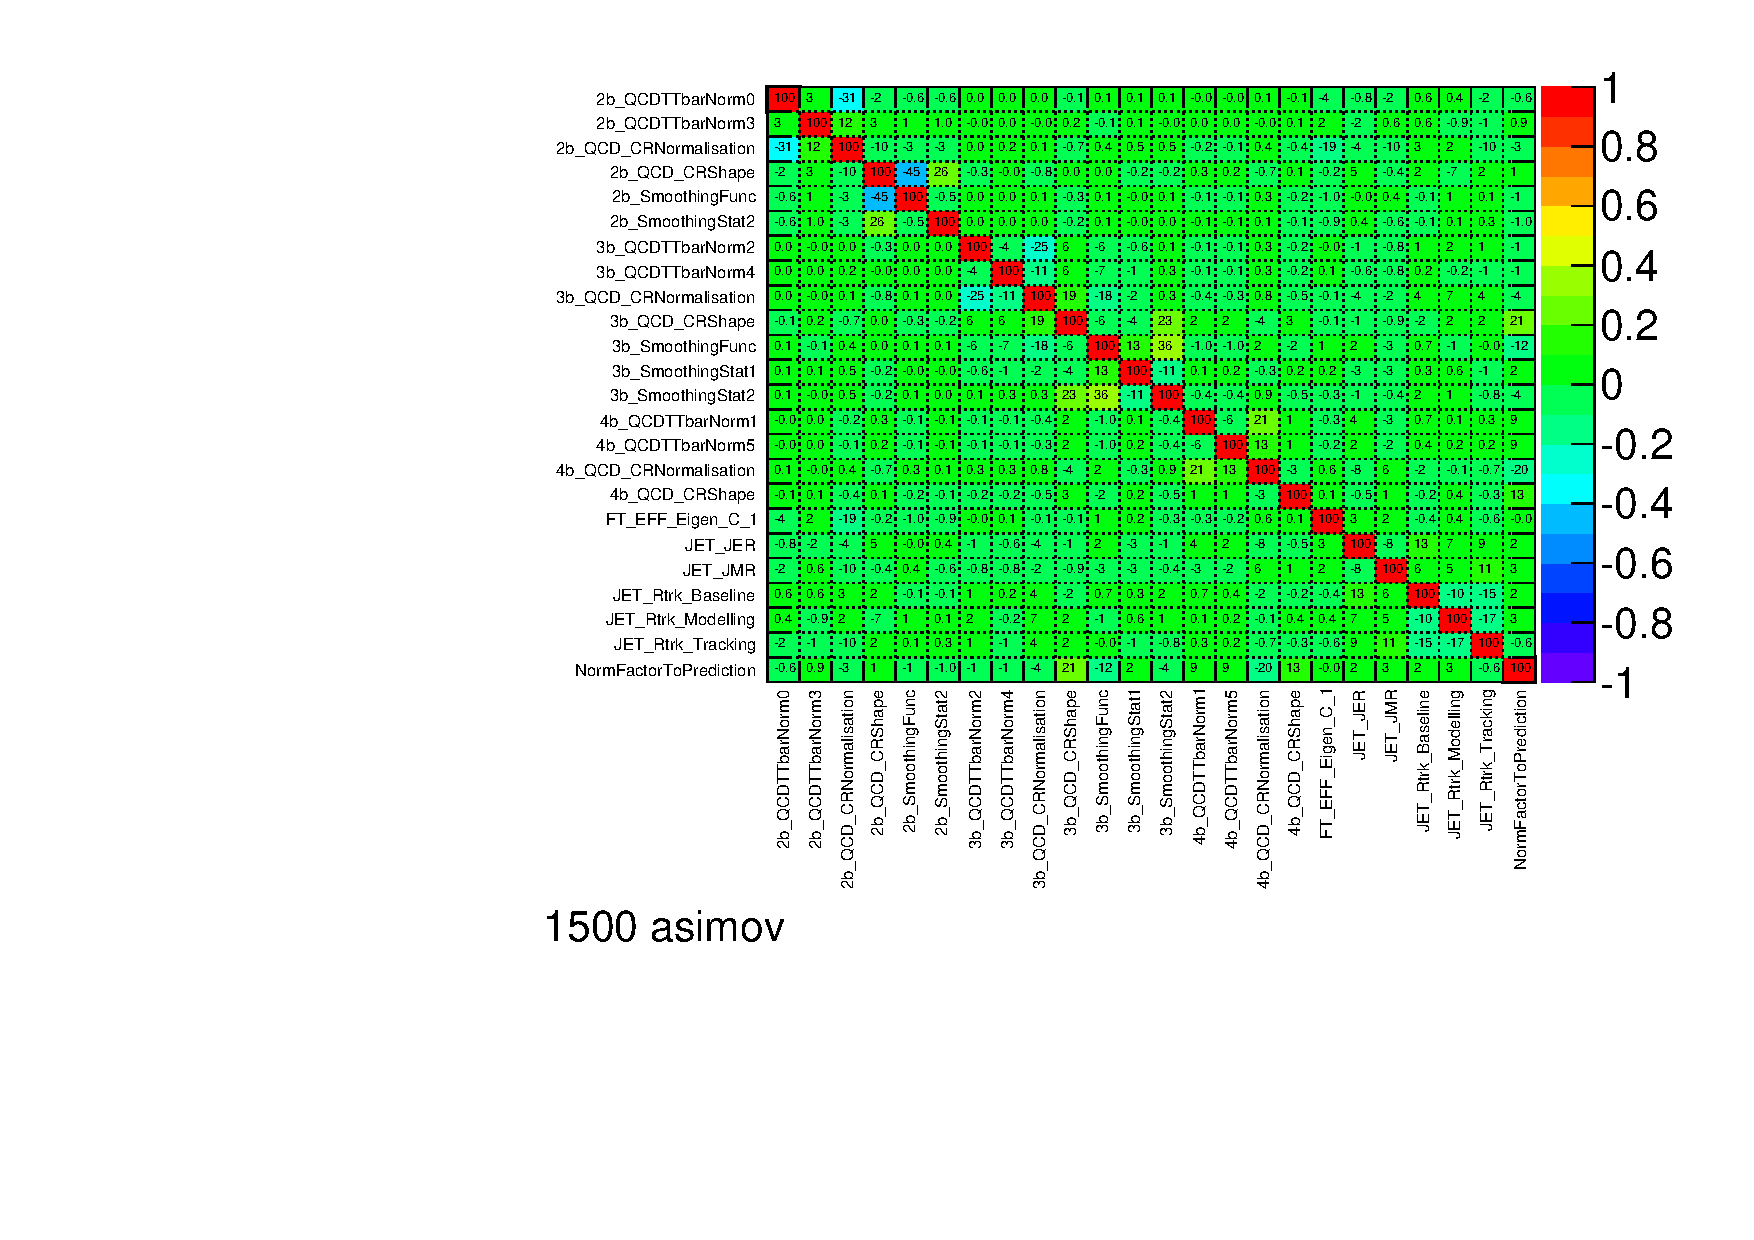
\includegraphics[angle=270, width=0.59\textwidth]{./figures/boosted/app-fitchecks/corr_1500_asimov.pdf} }
\caption{Pulls (a) and correlations (b) for the 1500 GeV mass point.}
\label{fig:fitchecks:pullcorr1500}
\end{center}
\end{figure*}

\begin{figure*}[htbp!]
\begin{center}
\subfloat[]{ 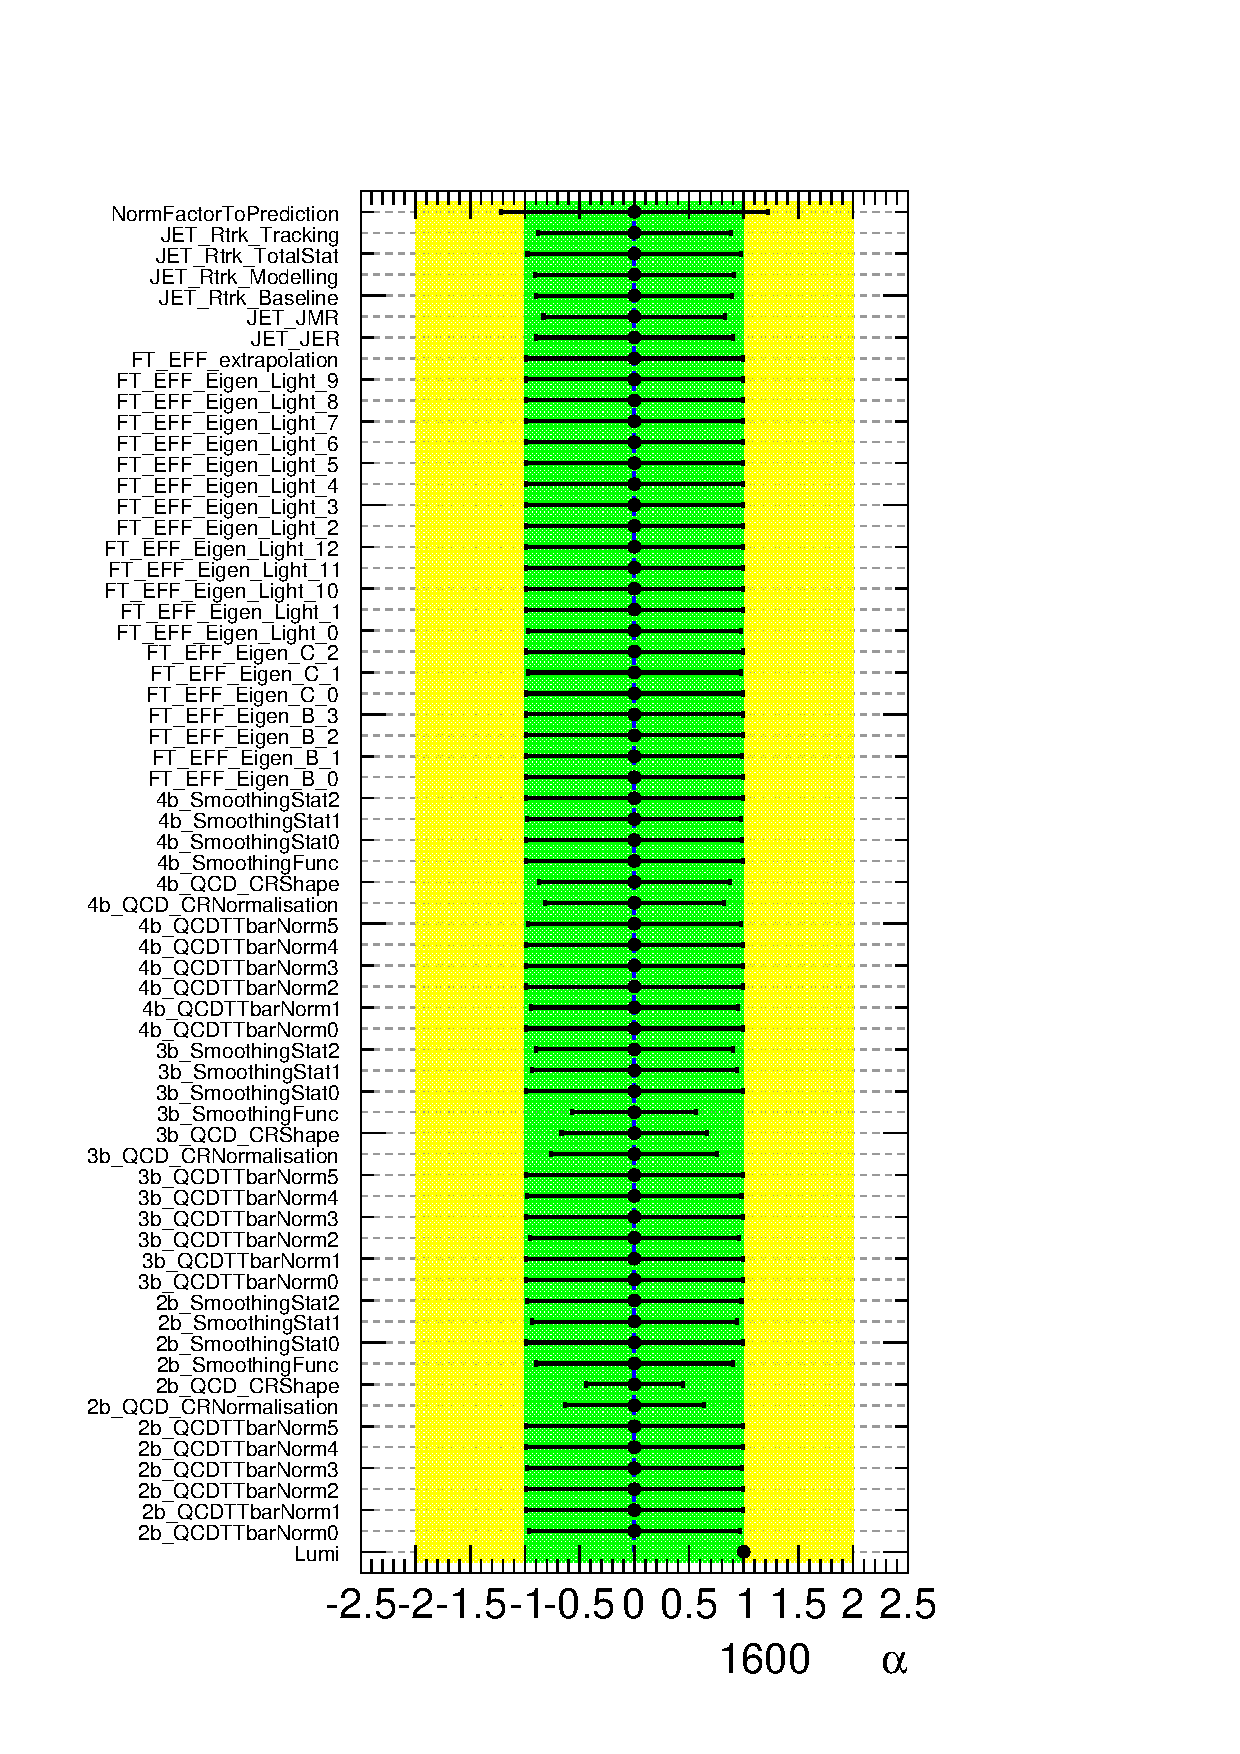
\includegraphics[angle=270, width=0.39\textwidth]{./figures/boosted/app-fitchecks/pulls_1600_asimov.pdf} }
\subfloat[]{ 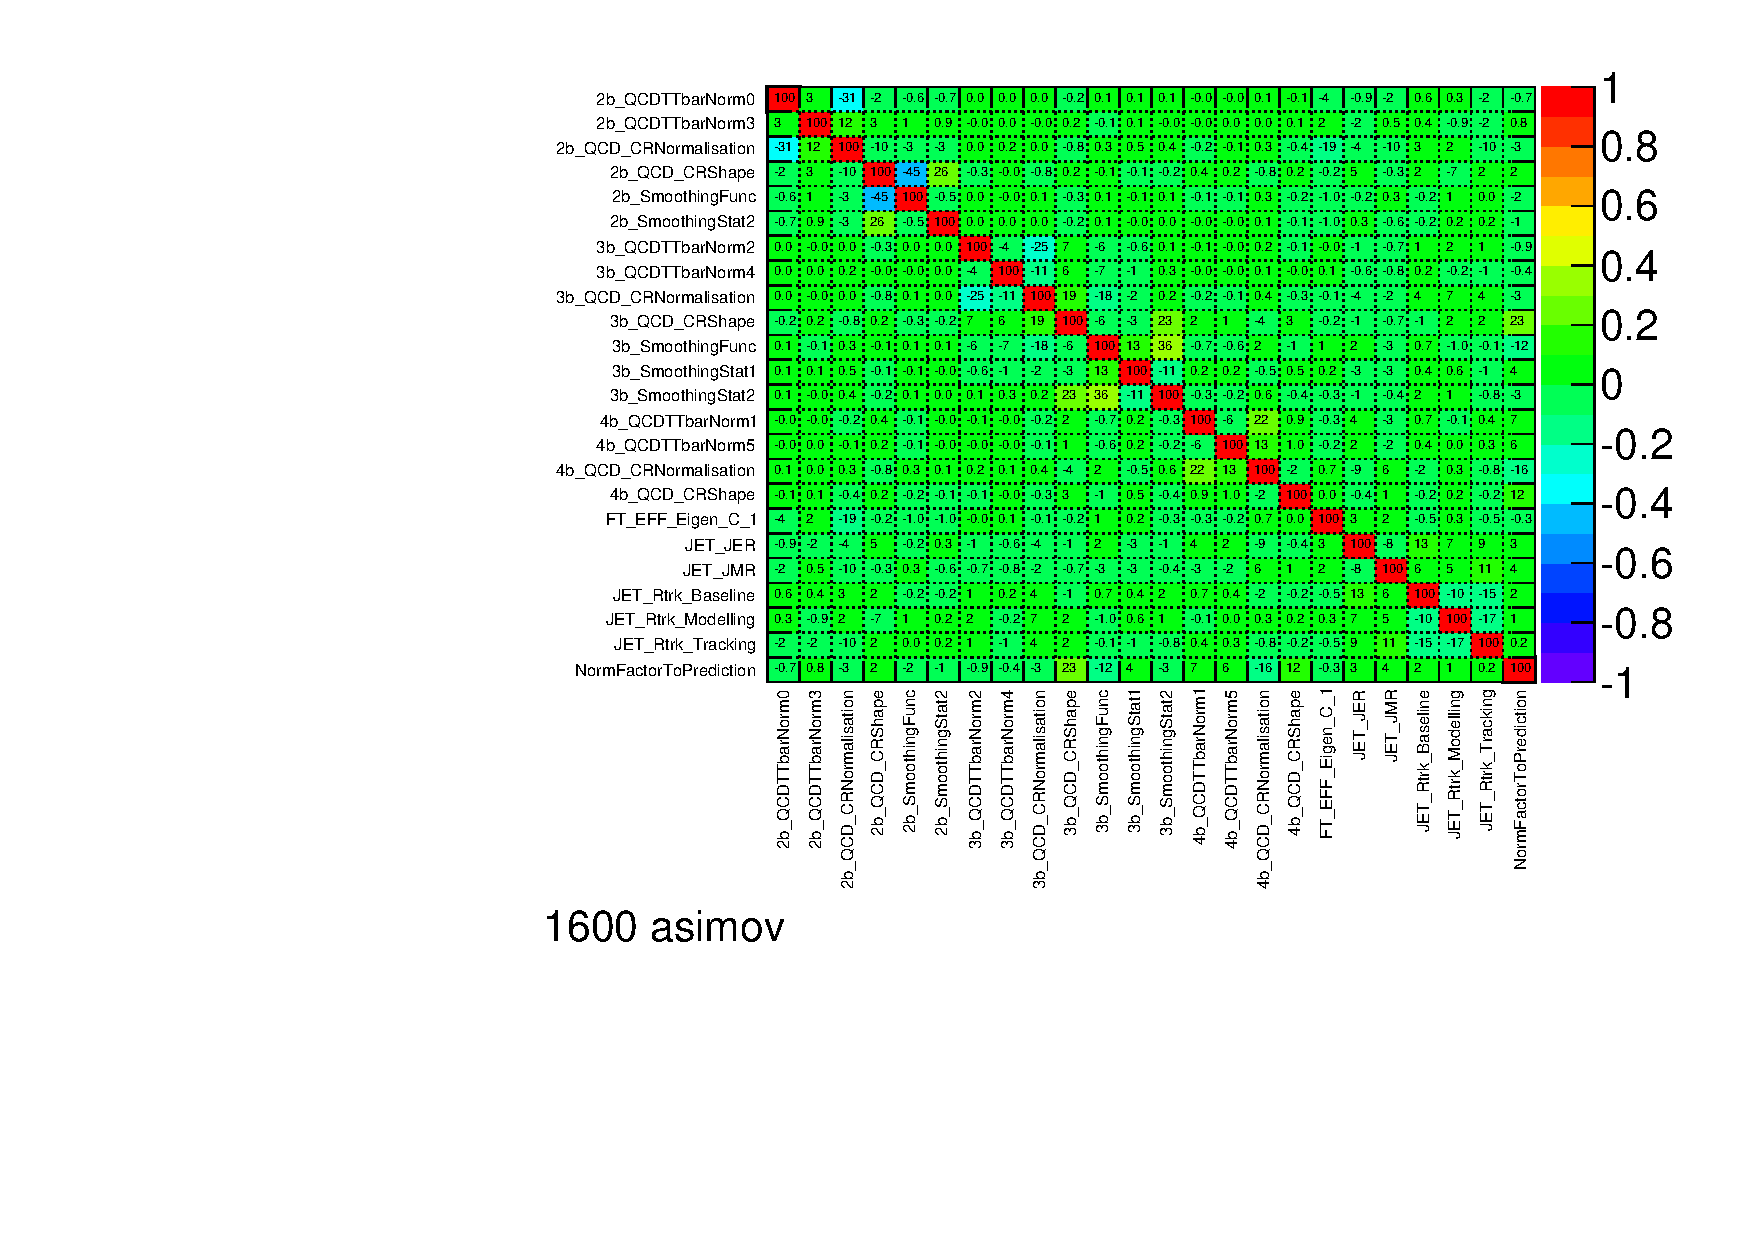
\includegraphics[angle=270, width=0.59\textwidth]{./figures/boosted/app-fitchecks/corr_1600_asimov.pdf} }
\caption{Pulls (a) and correlations (b) for the 1600 GeV mass point.}
\label{fig:fitchecks:pullcorr1600}
\end{center}
\end{figure*}

\begin{figure*}[htbp!]
\begin{center}
\subfloat[]{ 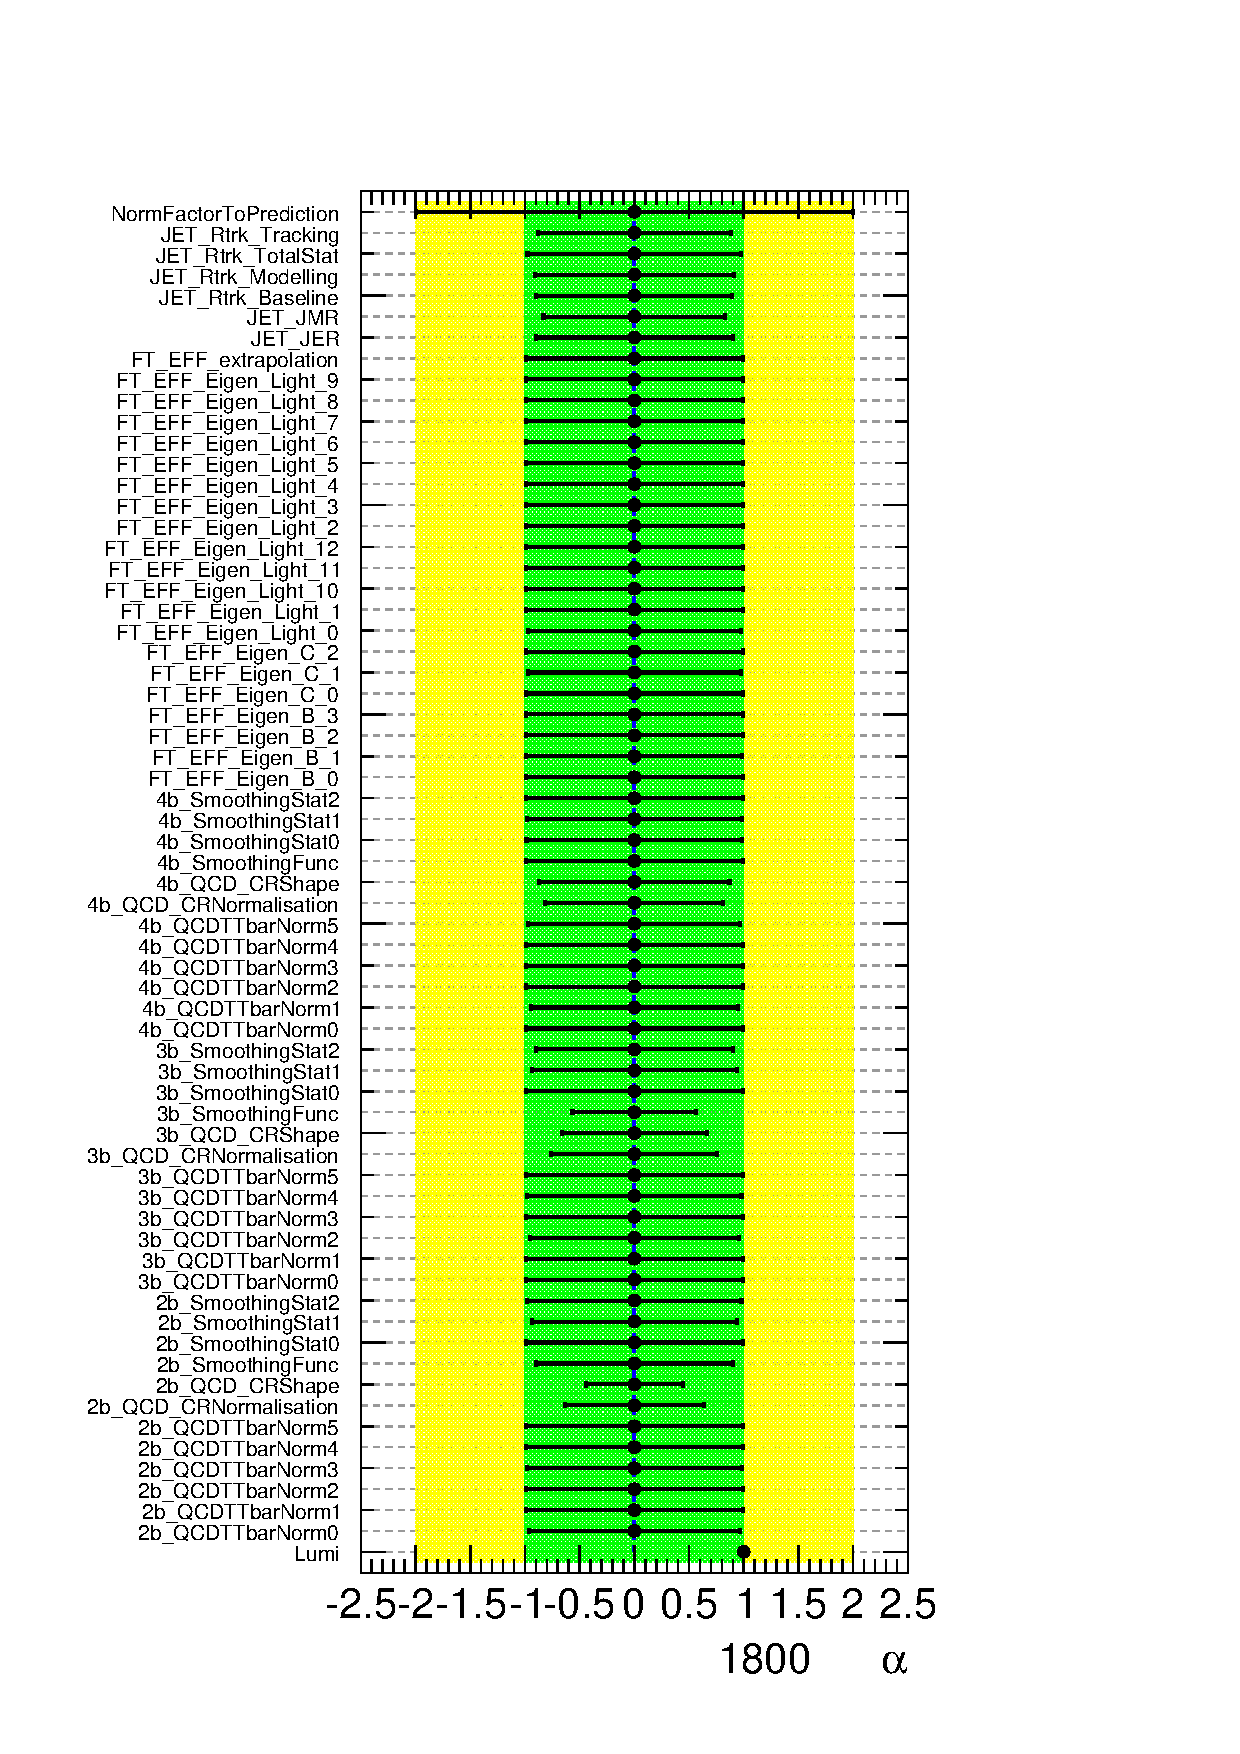
\includegraphics[angle=270, width=0.39\textwidth]{./figures/boosted/app-fitchecks/pulls_1800_asimov.pdf} }
\subfloat[]{ 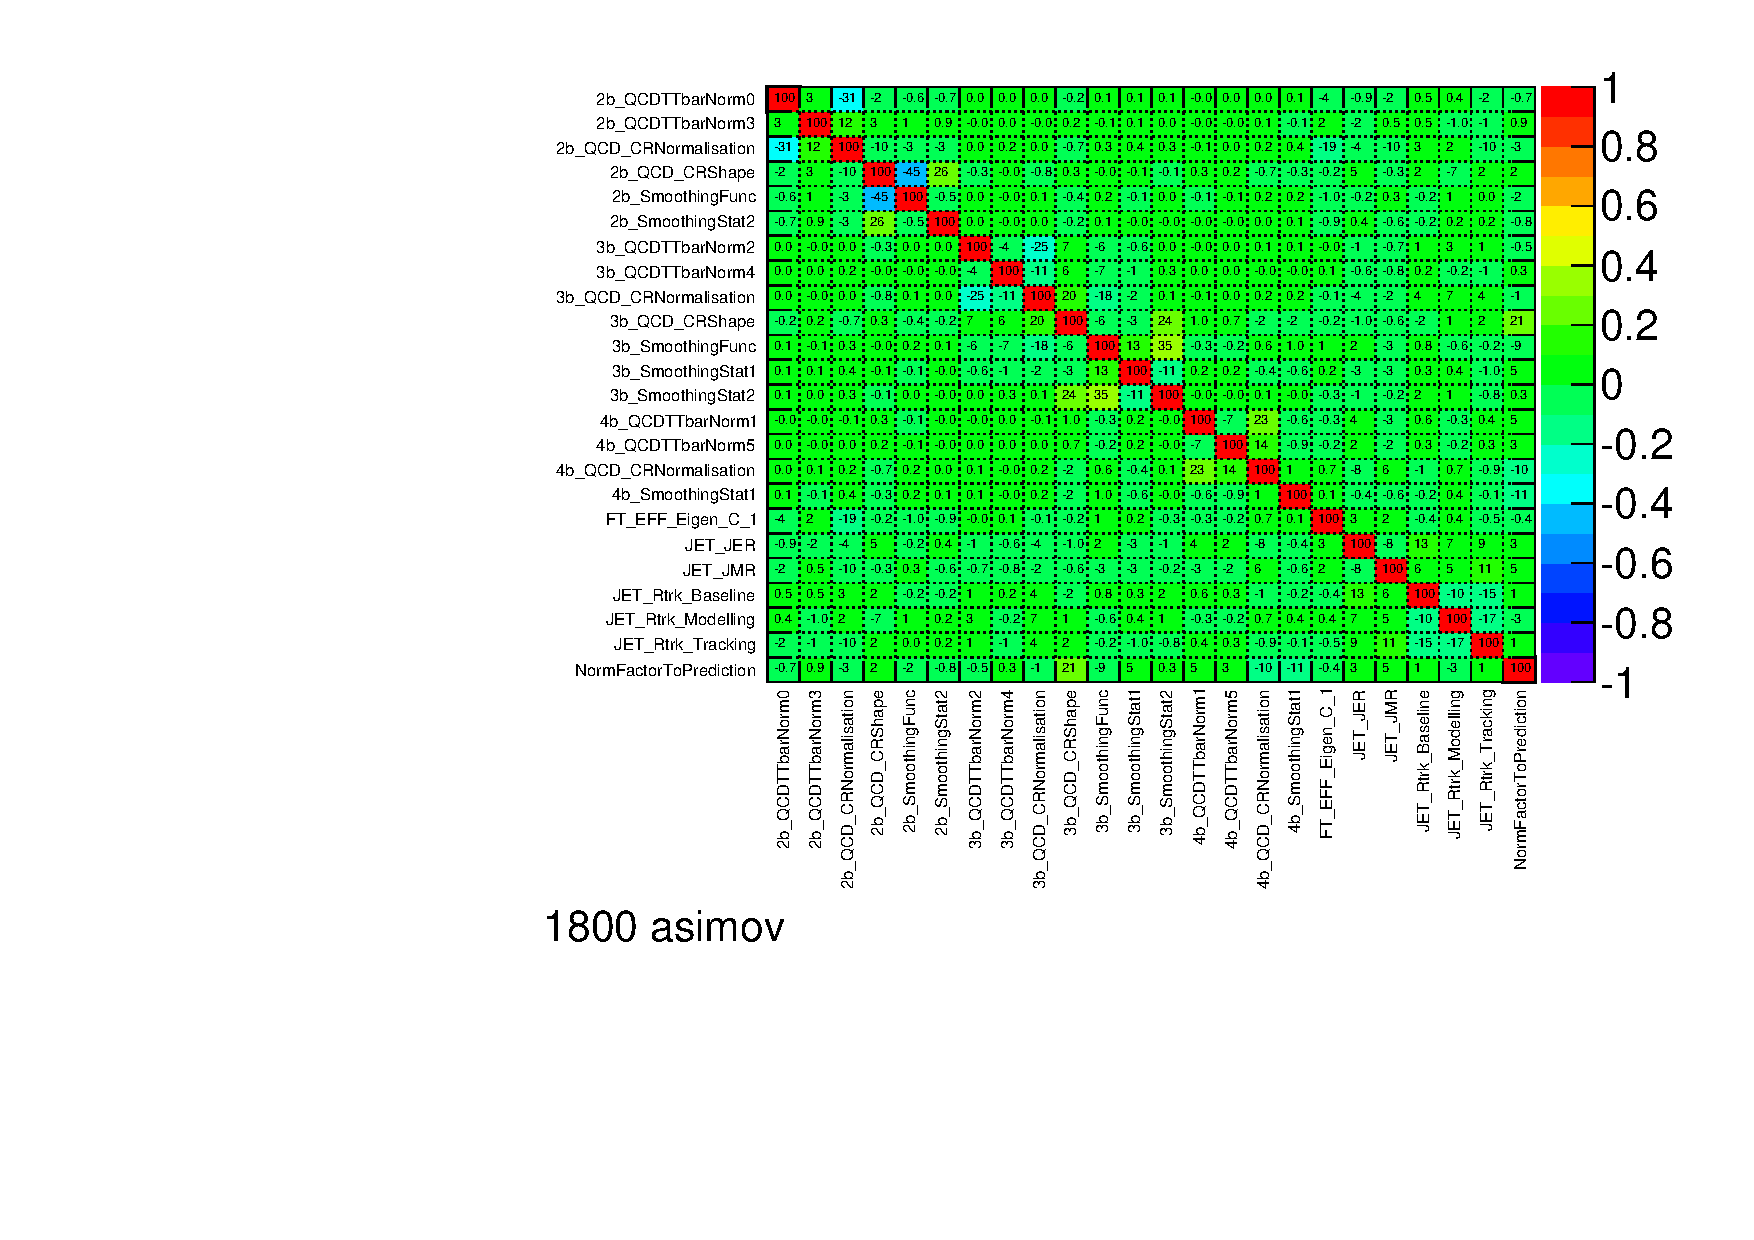
\includegraphics[angle=270, width=0.59\textwidth]{./figures/boosted/app-fitchecks/corr_1800_asimov.pdf} }
\caption{Pulls (a) and correlations (b) for the 1800 GeV mass point.}
\label{fig:fitchecks:pullcorr1800}
\end{center}
\end{figure*}

\begin{figure*}[htbp!]
\begin{center}
\subfloat[]{ 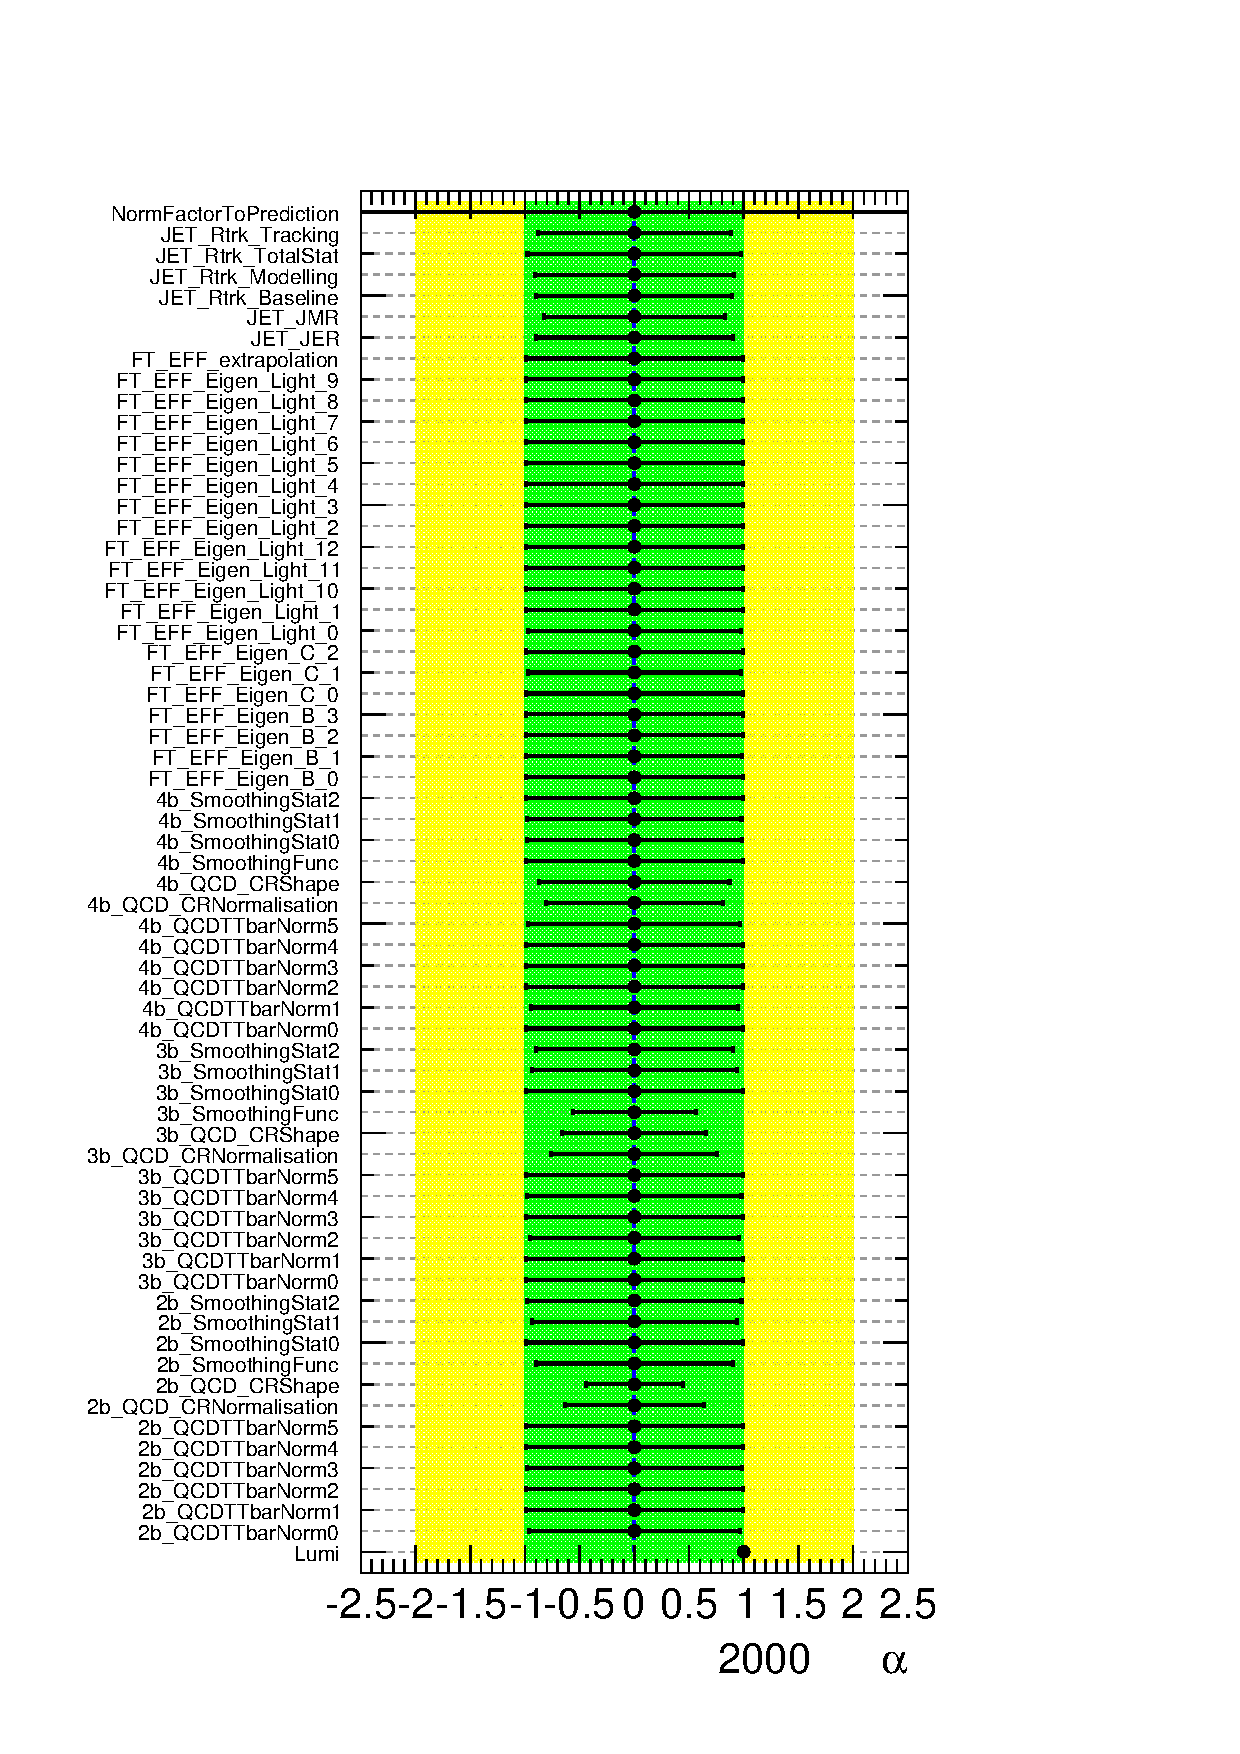
\includegraphics[angle=270, width=0.39\textwidth]{./figures/boosted/app-fitchecks/pulls_2000_asimov.pdf} }
\subfloat[]{ 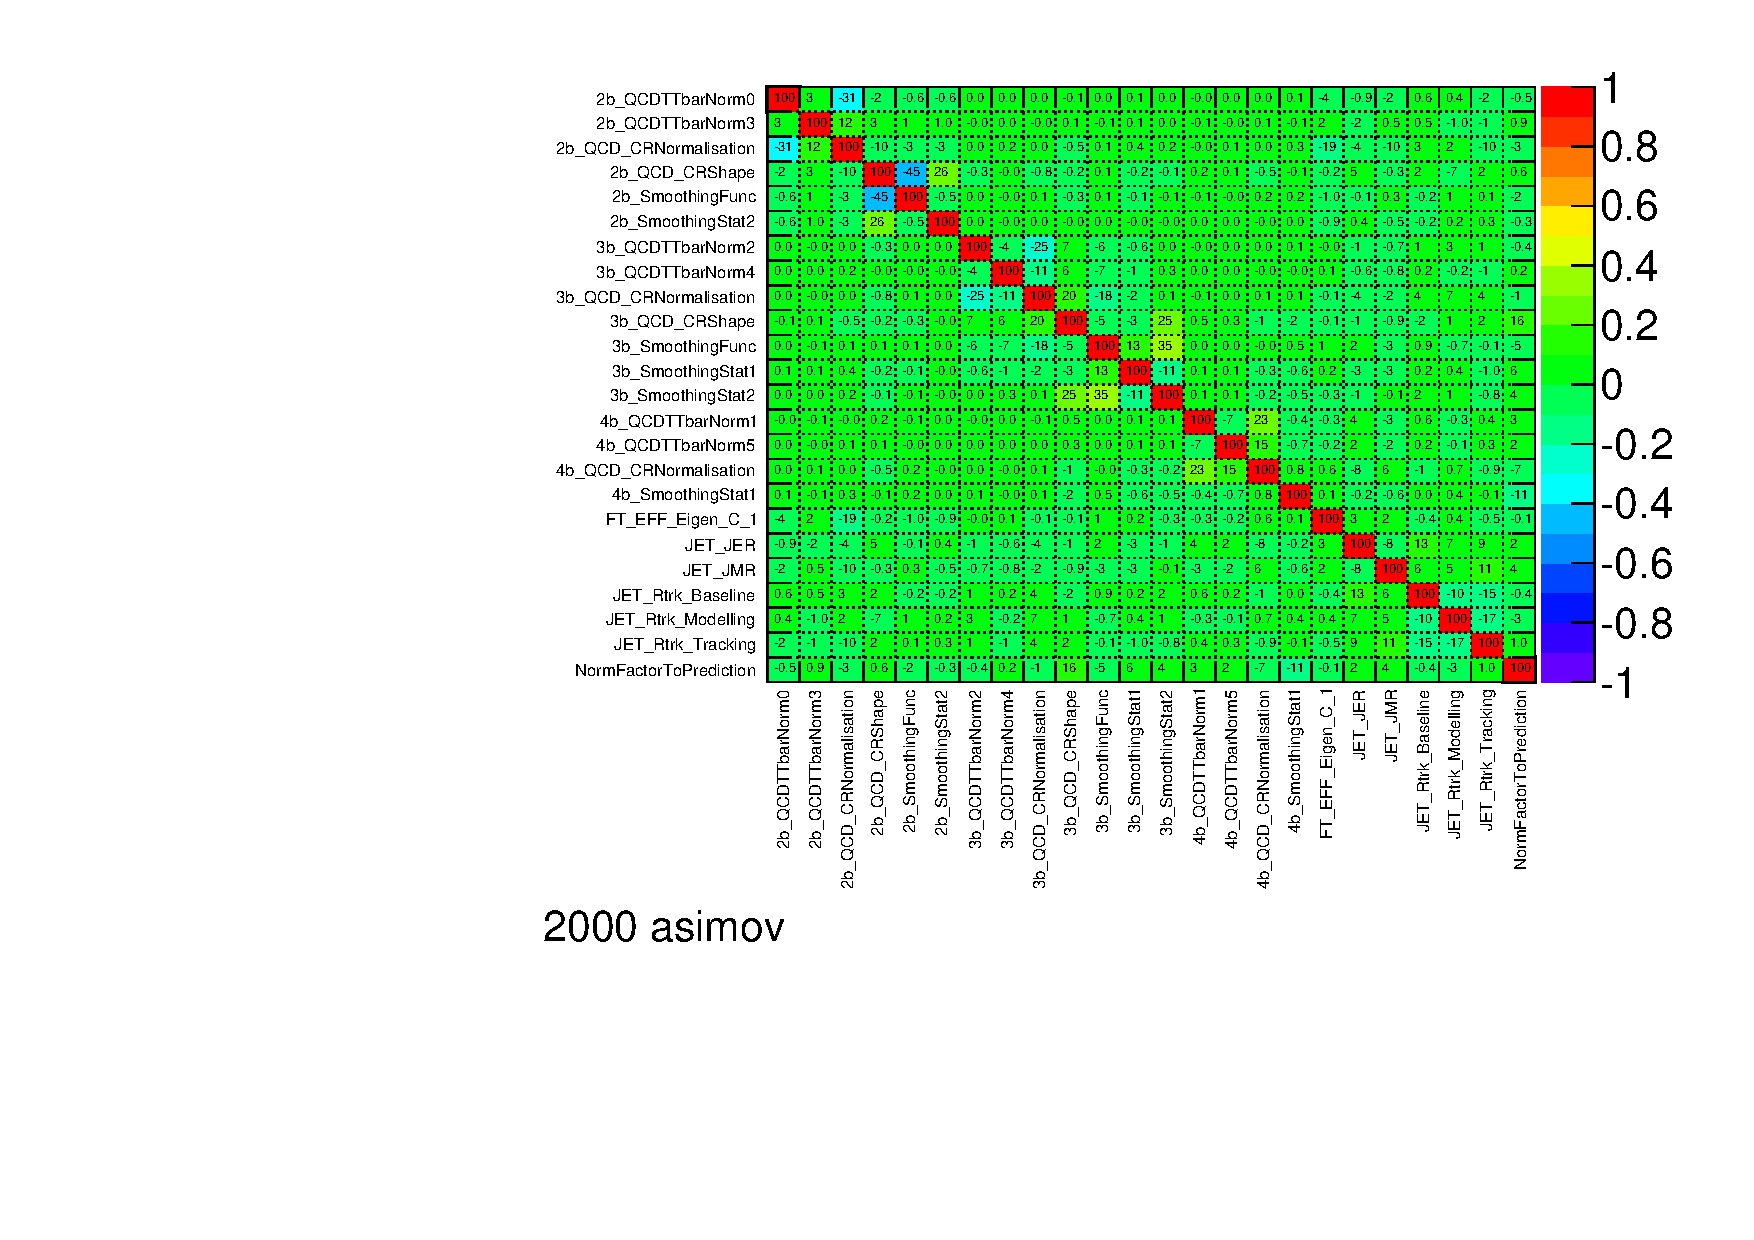
\includegraphics[angle=270, width=0.59\textwidth]{./figures/boosted/app-fitchecks/corr_2000_asimov.pdf} }
\caption{Pulls (a) and correlations (b) for the 2000 GeV mass point.}
\label{fig:fitchecks:pullcorr2000}
\end{center}
\end{figure*}

\begin{figure*}[htbp!]
\begin{center}
\subfloat[]{ 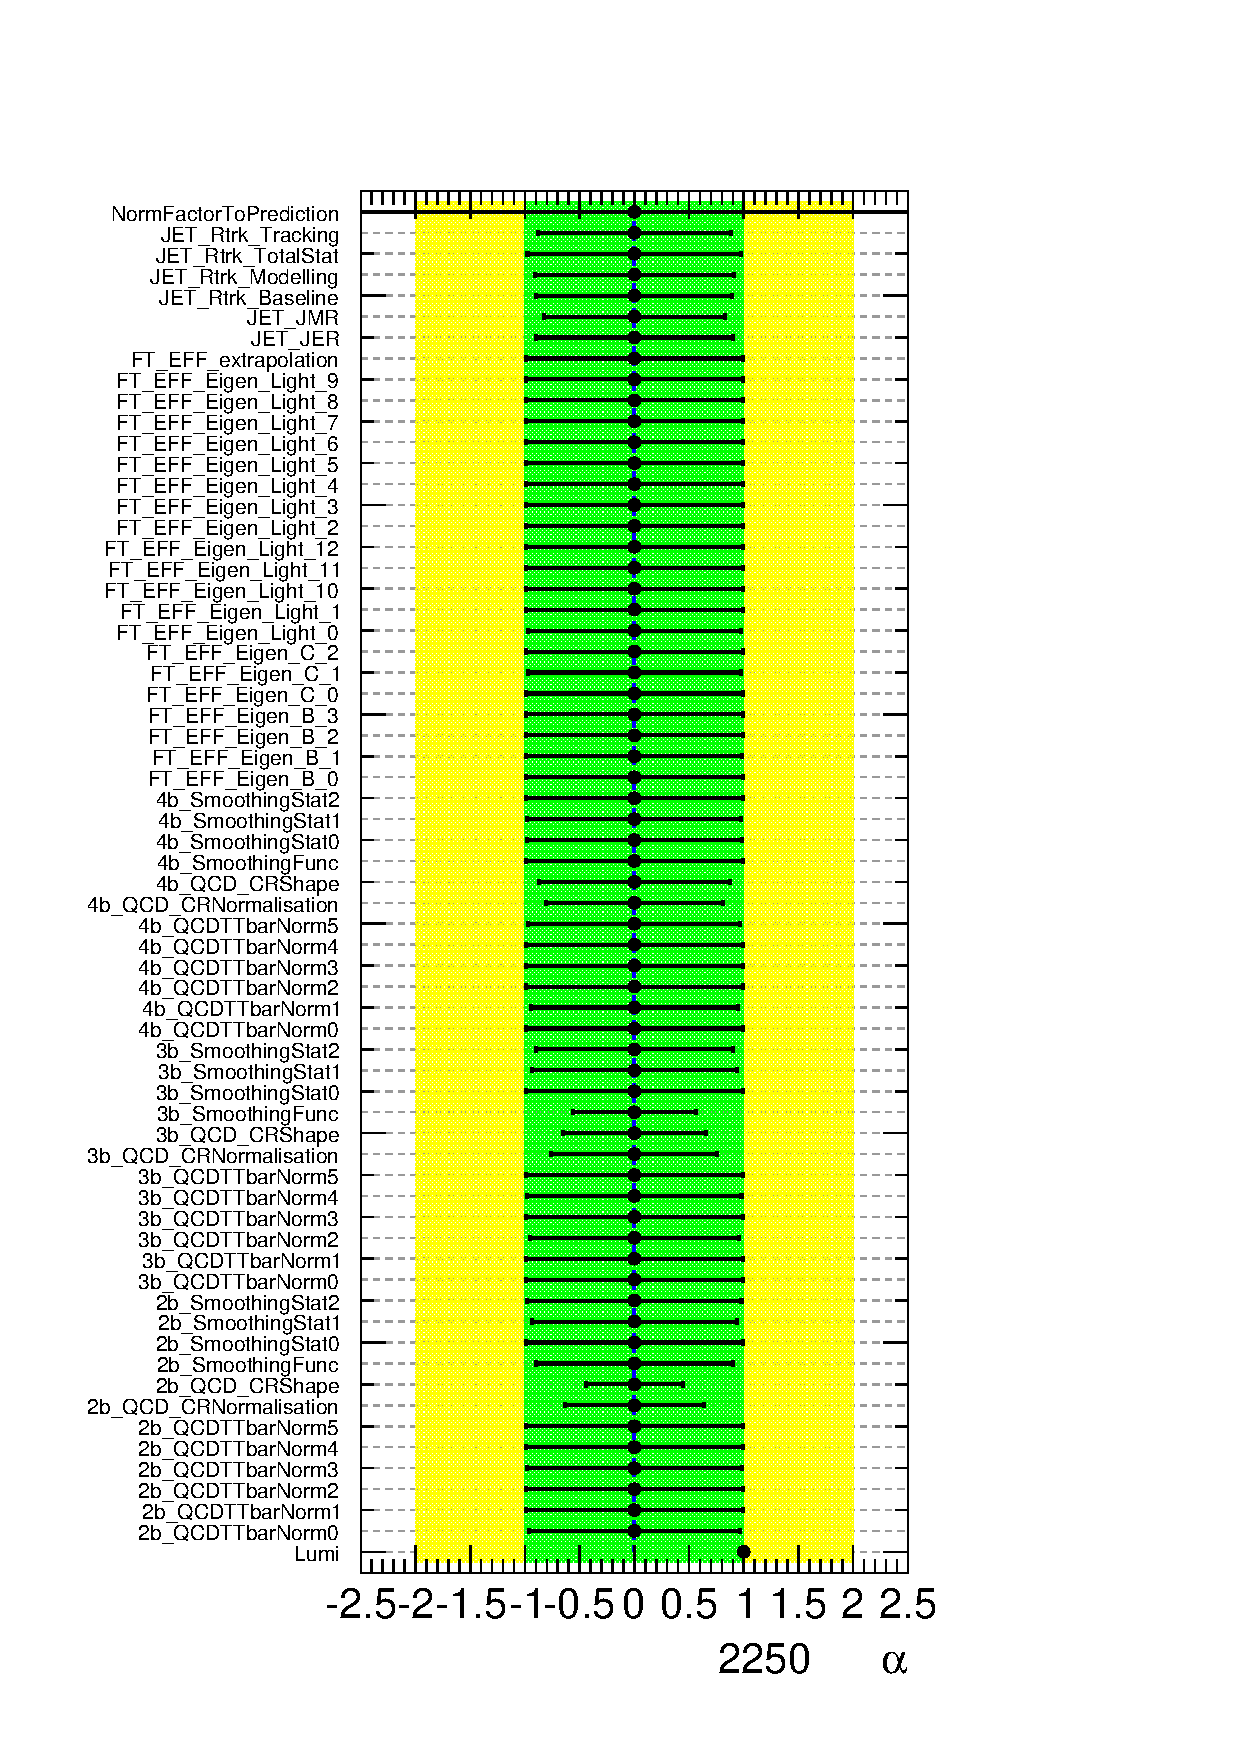
\includegraphics[angle=270, width=0.39\textwidth]{./figures/boosted/app-fitchecks/pulls_2250_asimov.pdf} }
\subfloat[]{ 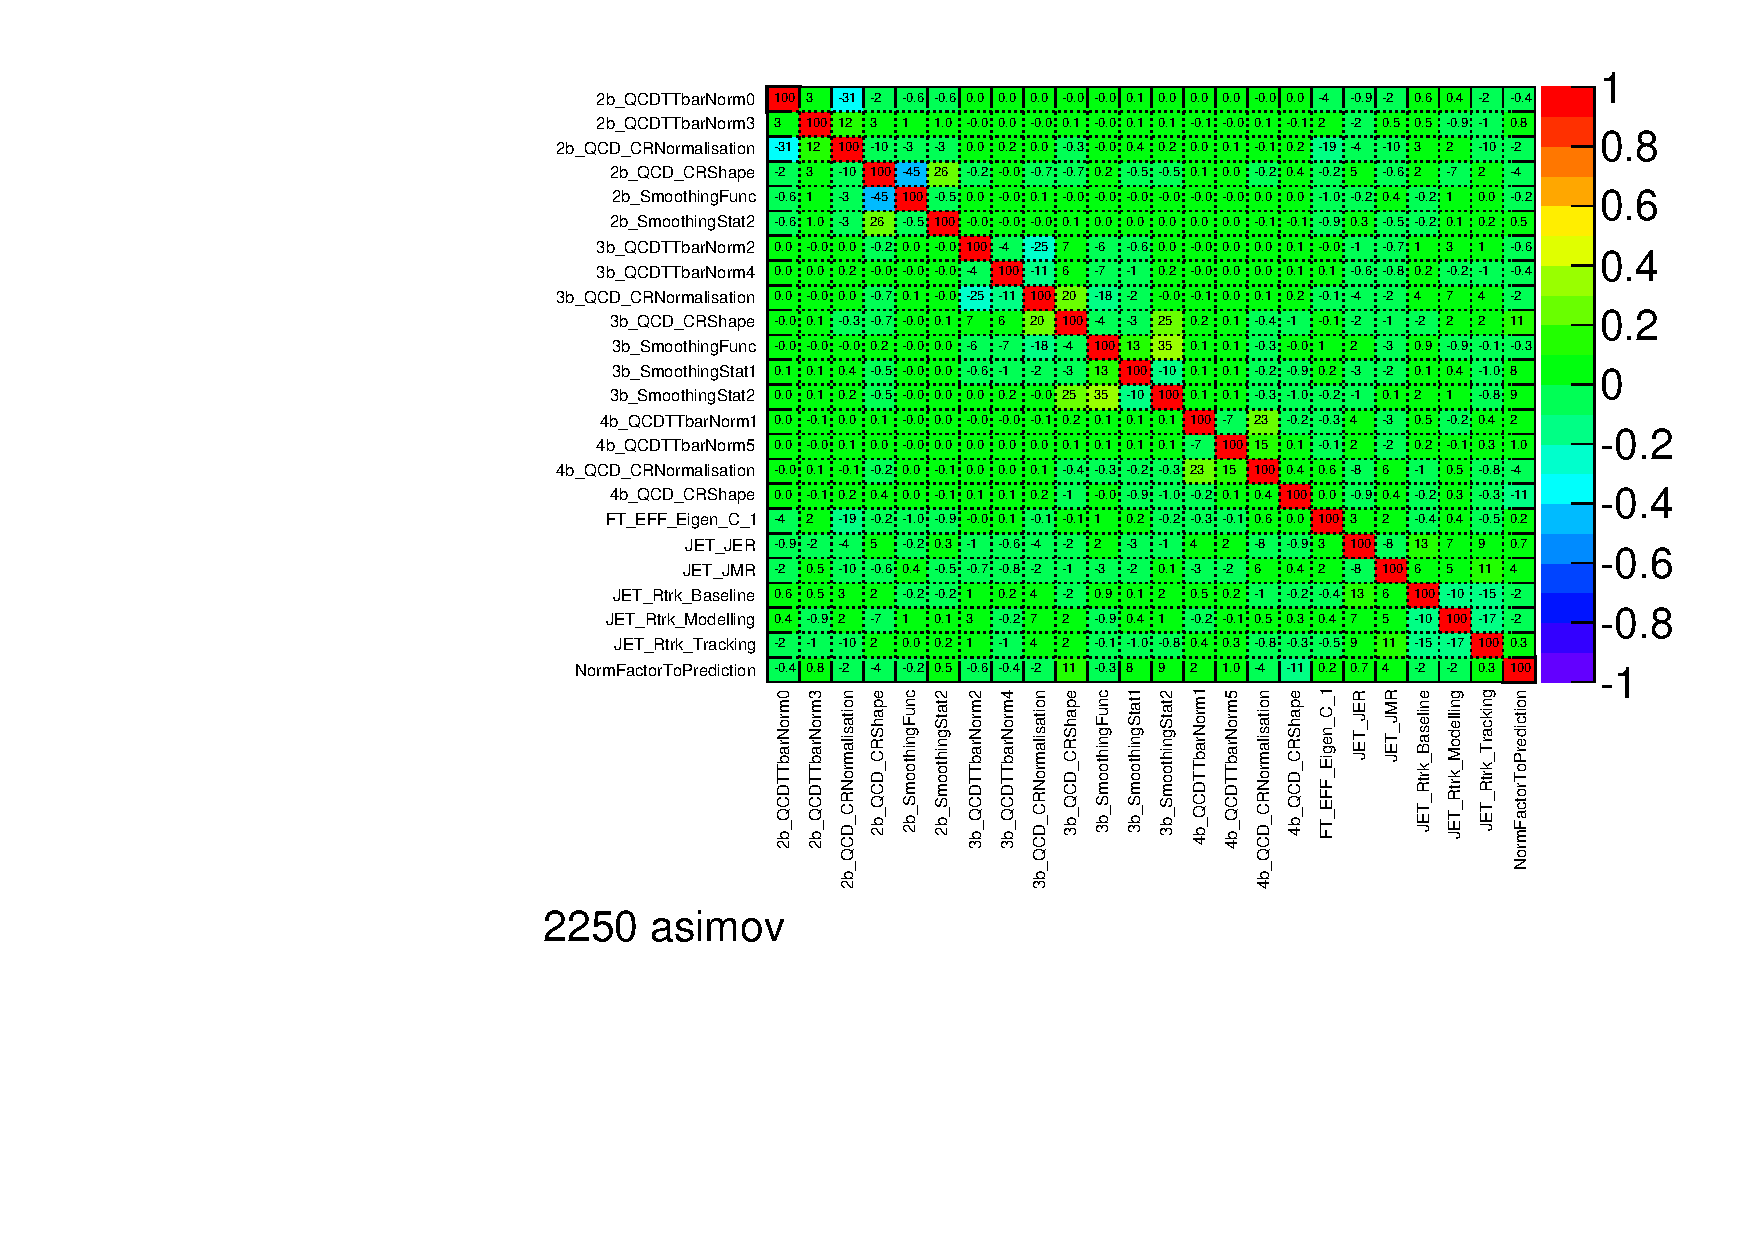
\includegraphics[angle=270, width=0.59\textwidth]{./figures/boosted/app-fitchecks/corr_2250_asimov.pdf} }
\caption{Pulls (a) and correlations (b) for the 2250 GeV mass point.}
\label{fig:fitchecks:pullcorr2250}
\end{center}
\end{figure*}

\begin{figure*}[htbp!]
\begin{center}
\subfloat[]{ 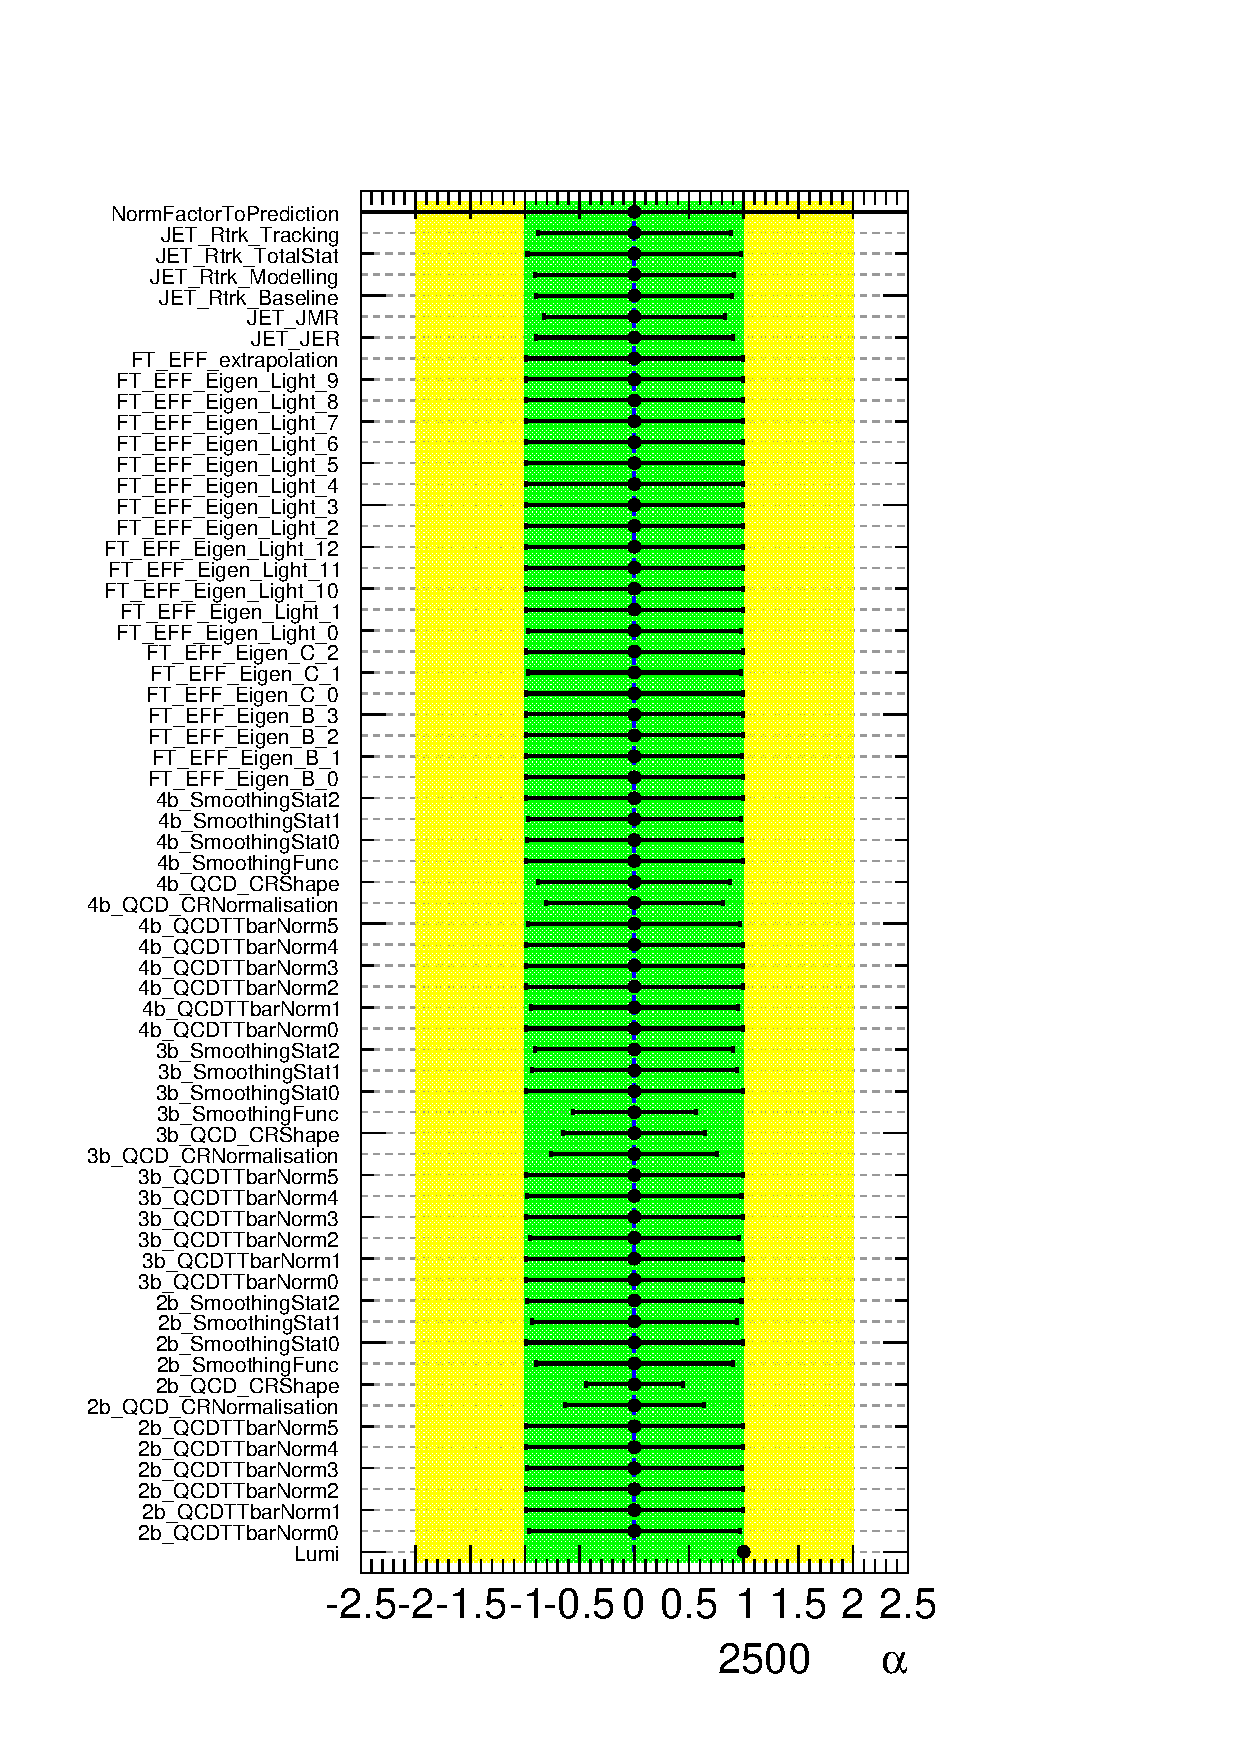
\includegraphics[angle=270, width=0.39\textwidth]{./figures/boosted/app-fitchecks/pulls_2500_asimov.pdf} }
\subfloat[]{ 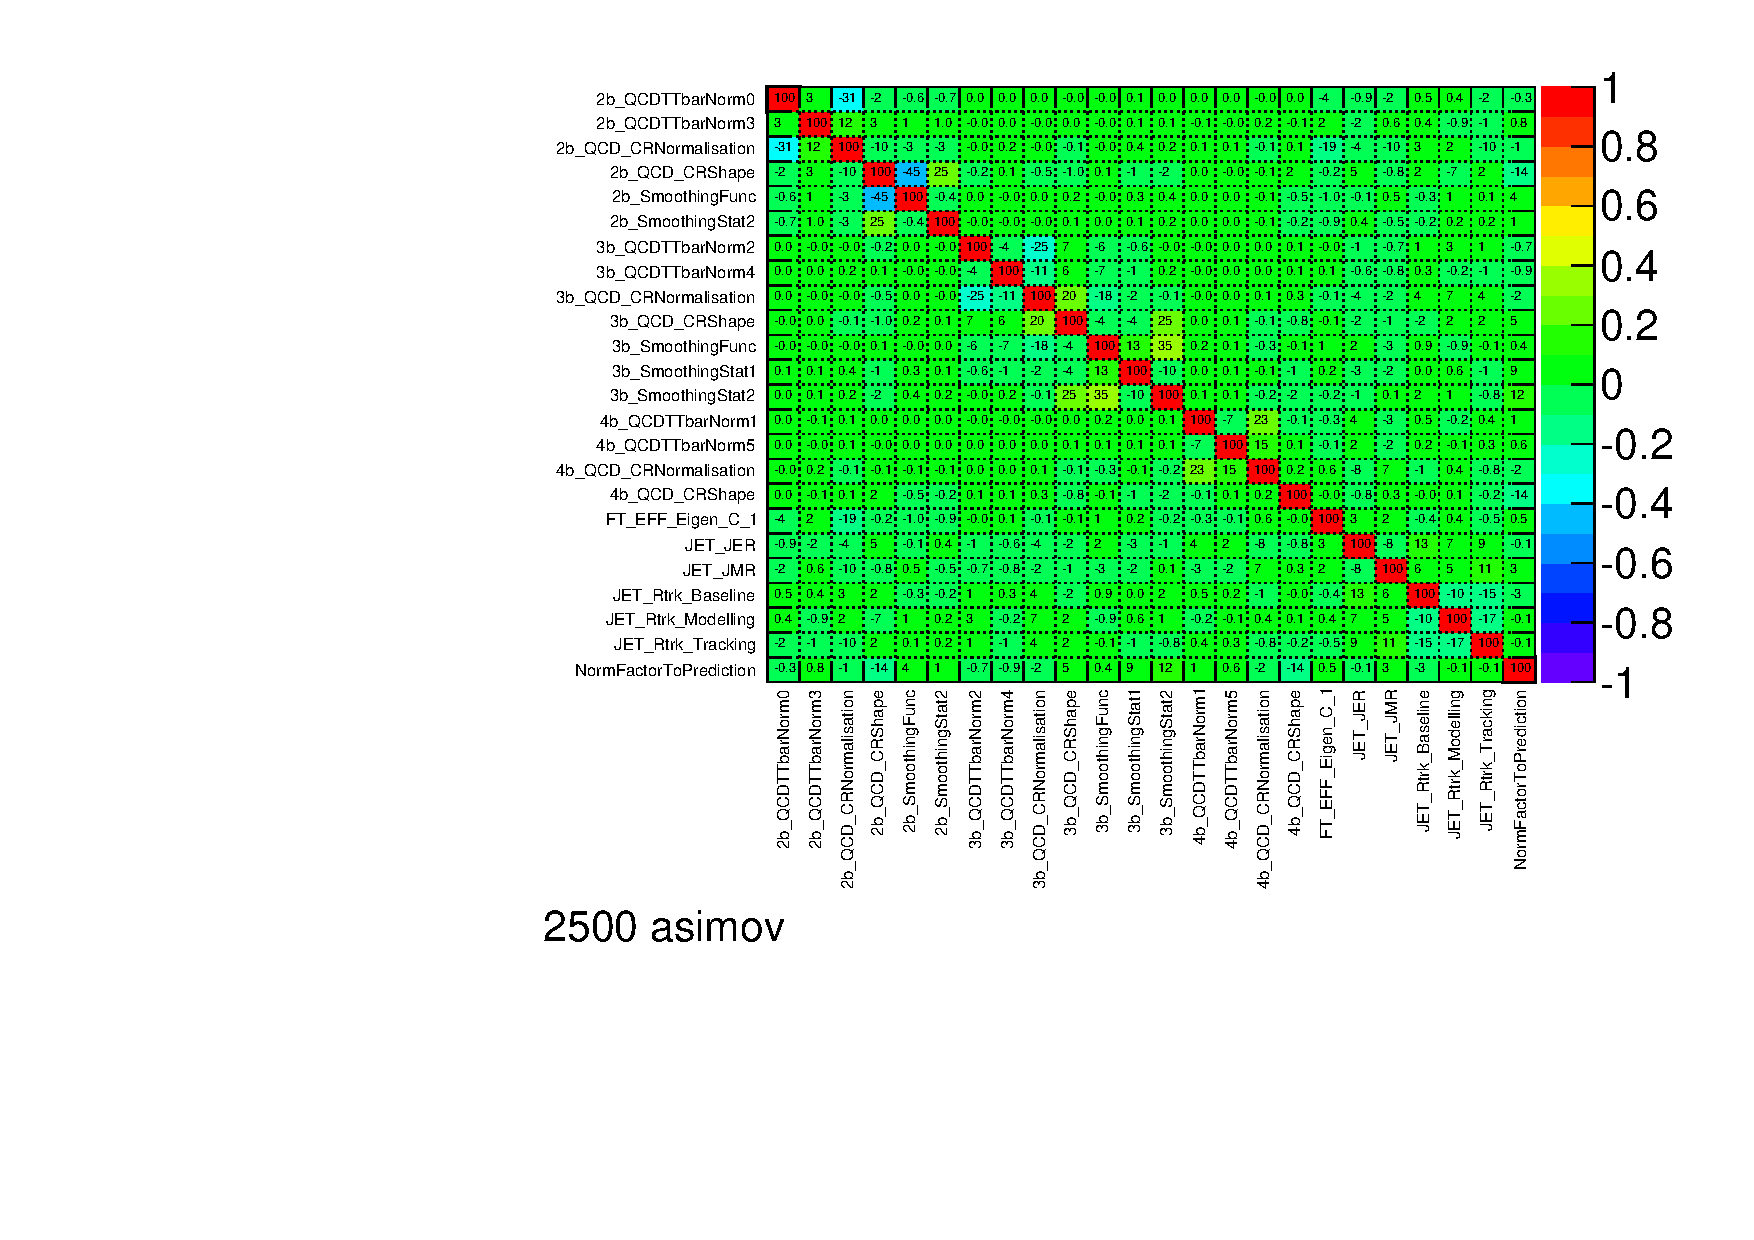
\includegraphics[angle=270, width=0.59\textwidth]{./figures/boosted/app-fitchecks/corr_2500_asimov.pdf} }
\caption{Pulls (a) and correlations (b) for the 2500 GeV mass point.}
\label{fig:fitchecks:pullcorr2500}
\end{center}
\end{figure*}

\begin{figure*}[htbp!]
\begin{center}
\subfloat[]{ 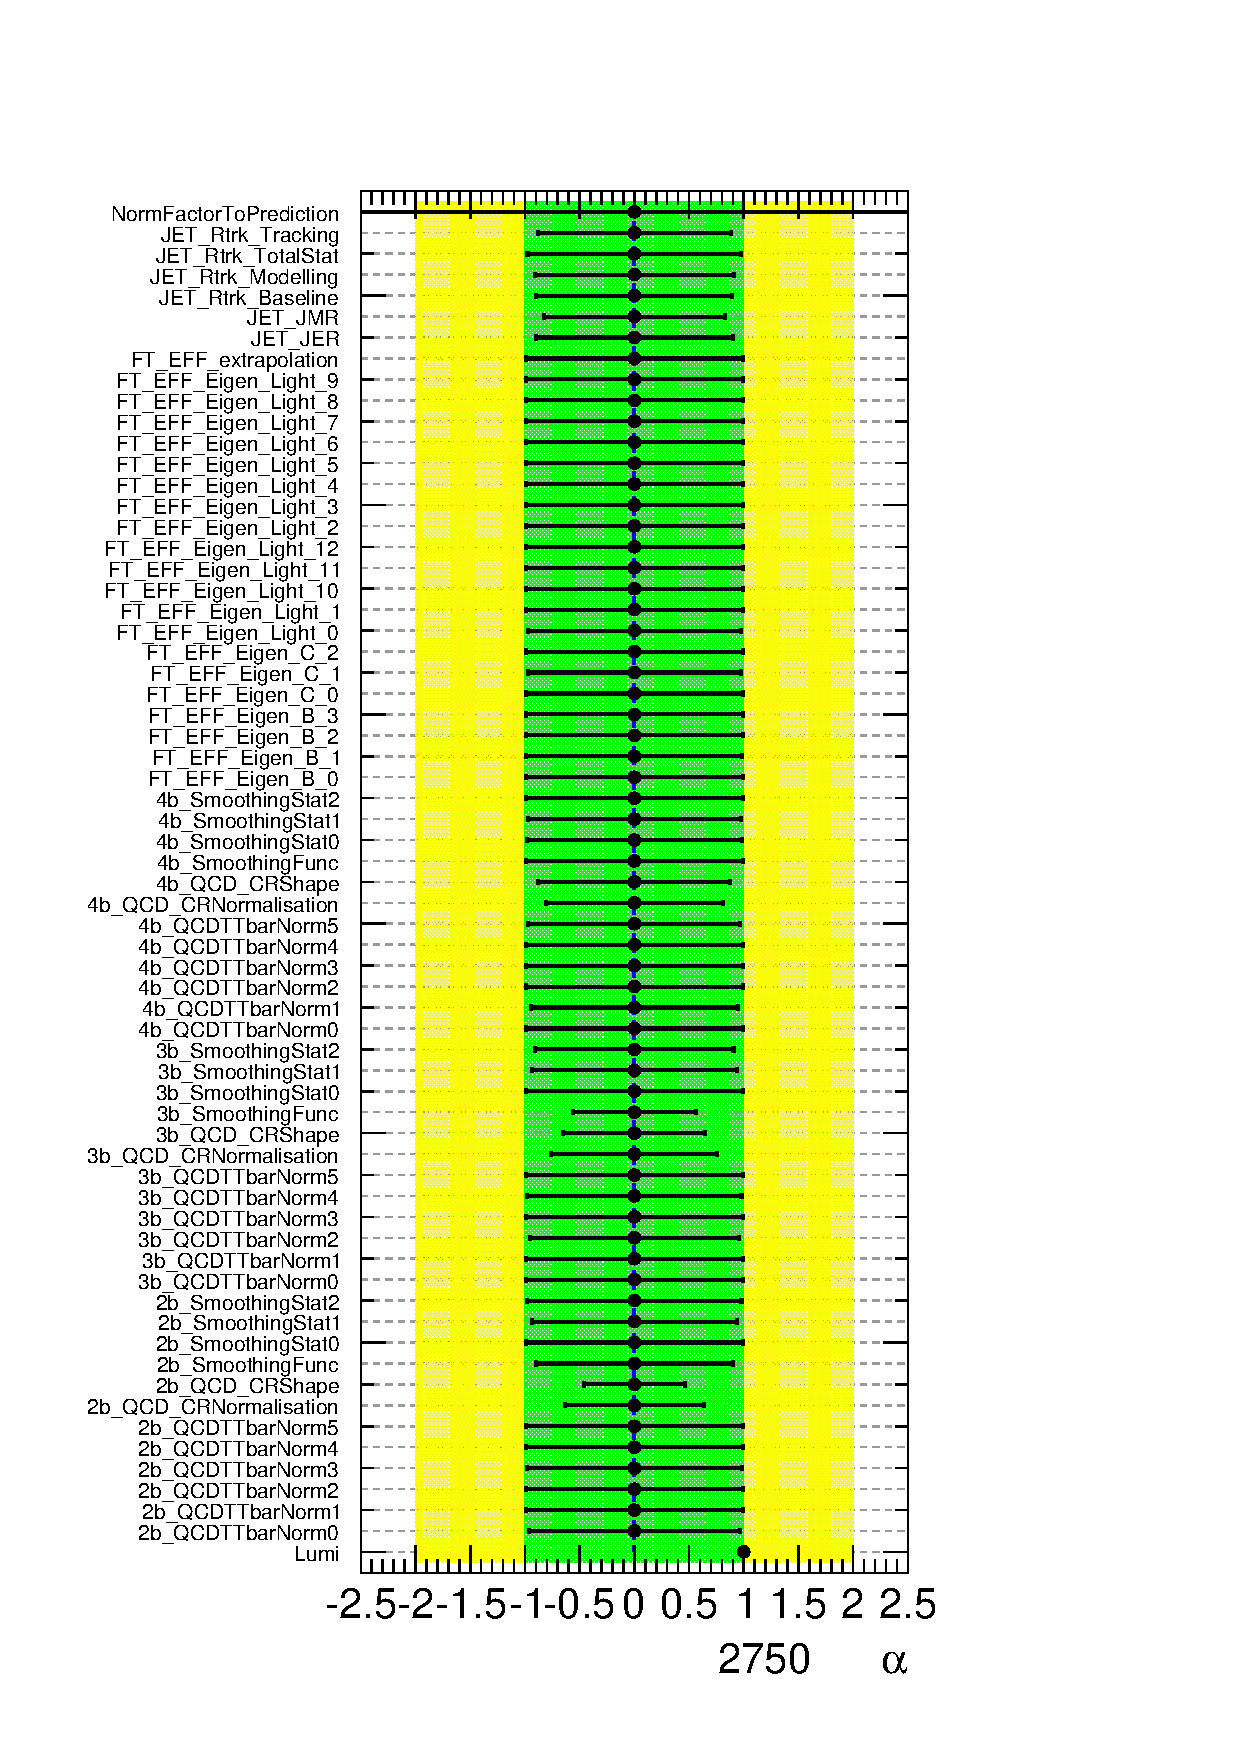
\includegraphics[angle=270, width=0.39\textwidth]{./figures/boosted/app-fitchecks/pulls_2750_asimov.pdf} }
\subfloat[]{ 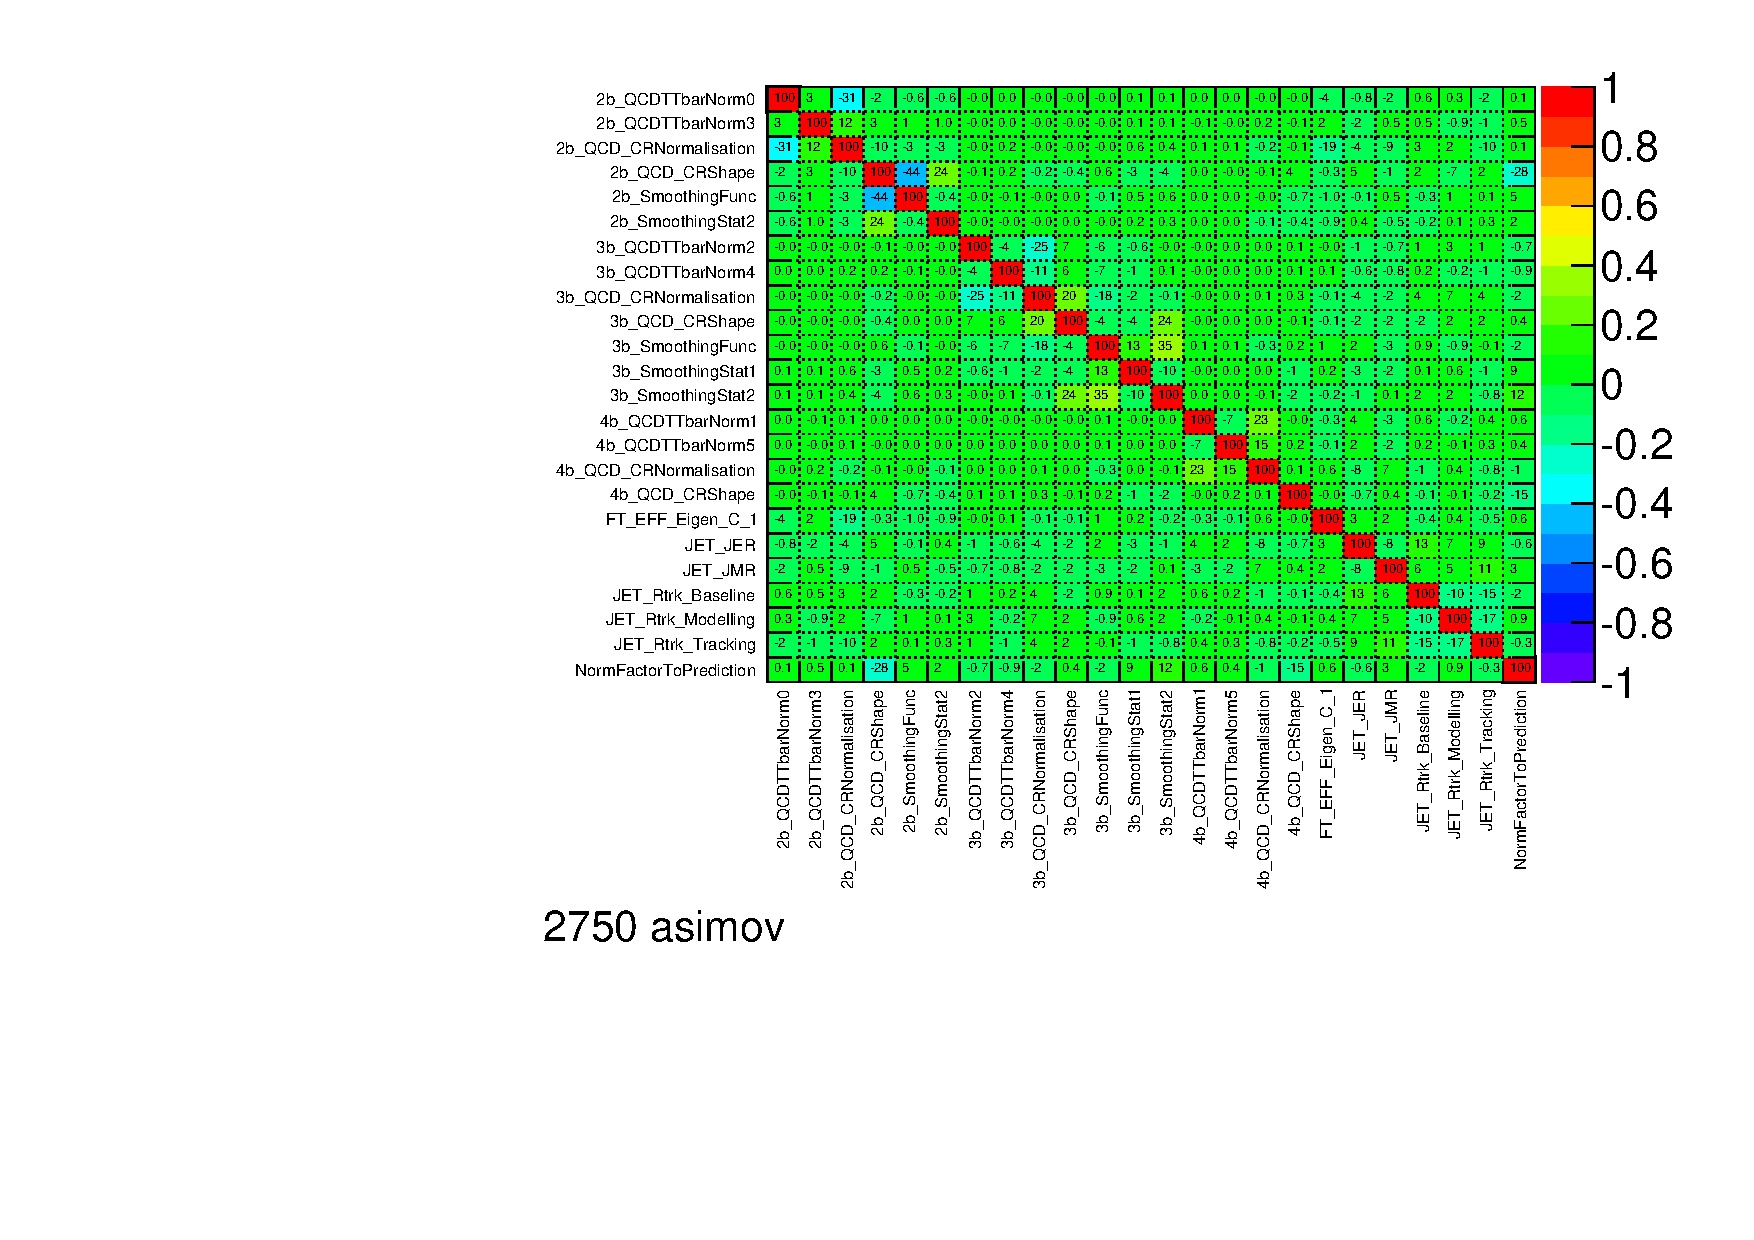
\includegraphics[angle=270, width=0.59\textwidth]{./figures/boosted/app-fitchecks/corr_2750_asimov.pdf} }
\caption{Pulls (a) and correlations (b) for the 2750 GeV mass point.}
\label{fig:fitchecks:pullcorr2750}
\end{center}
\end{figure*}

\begin{figure*}[htbp!]
\begin{center}
\subfloat[]{ 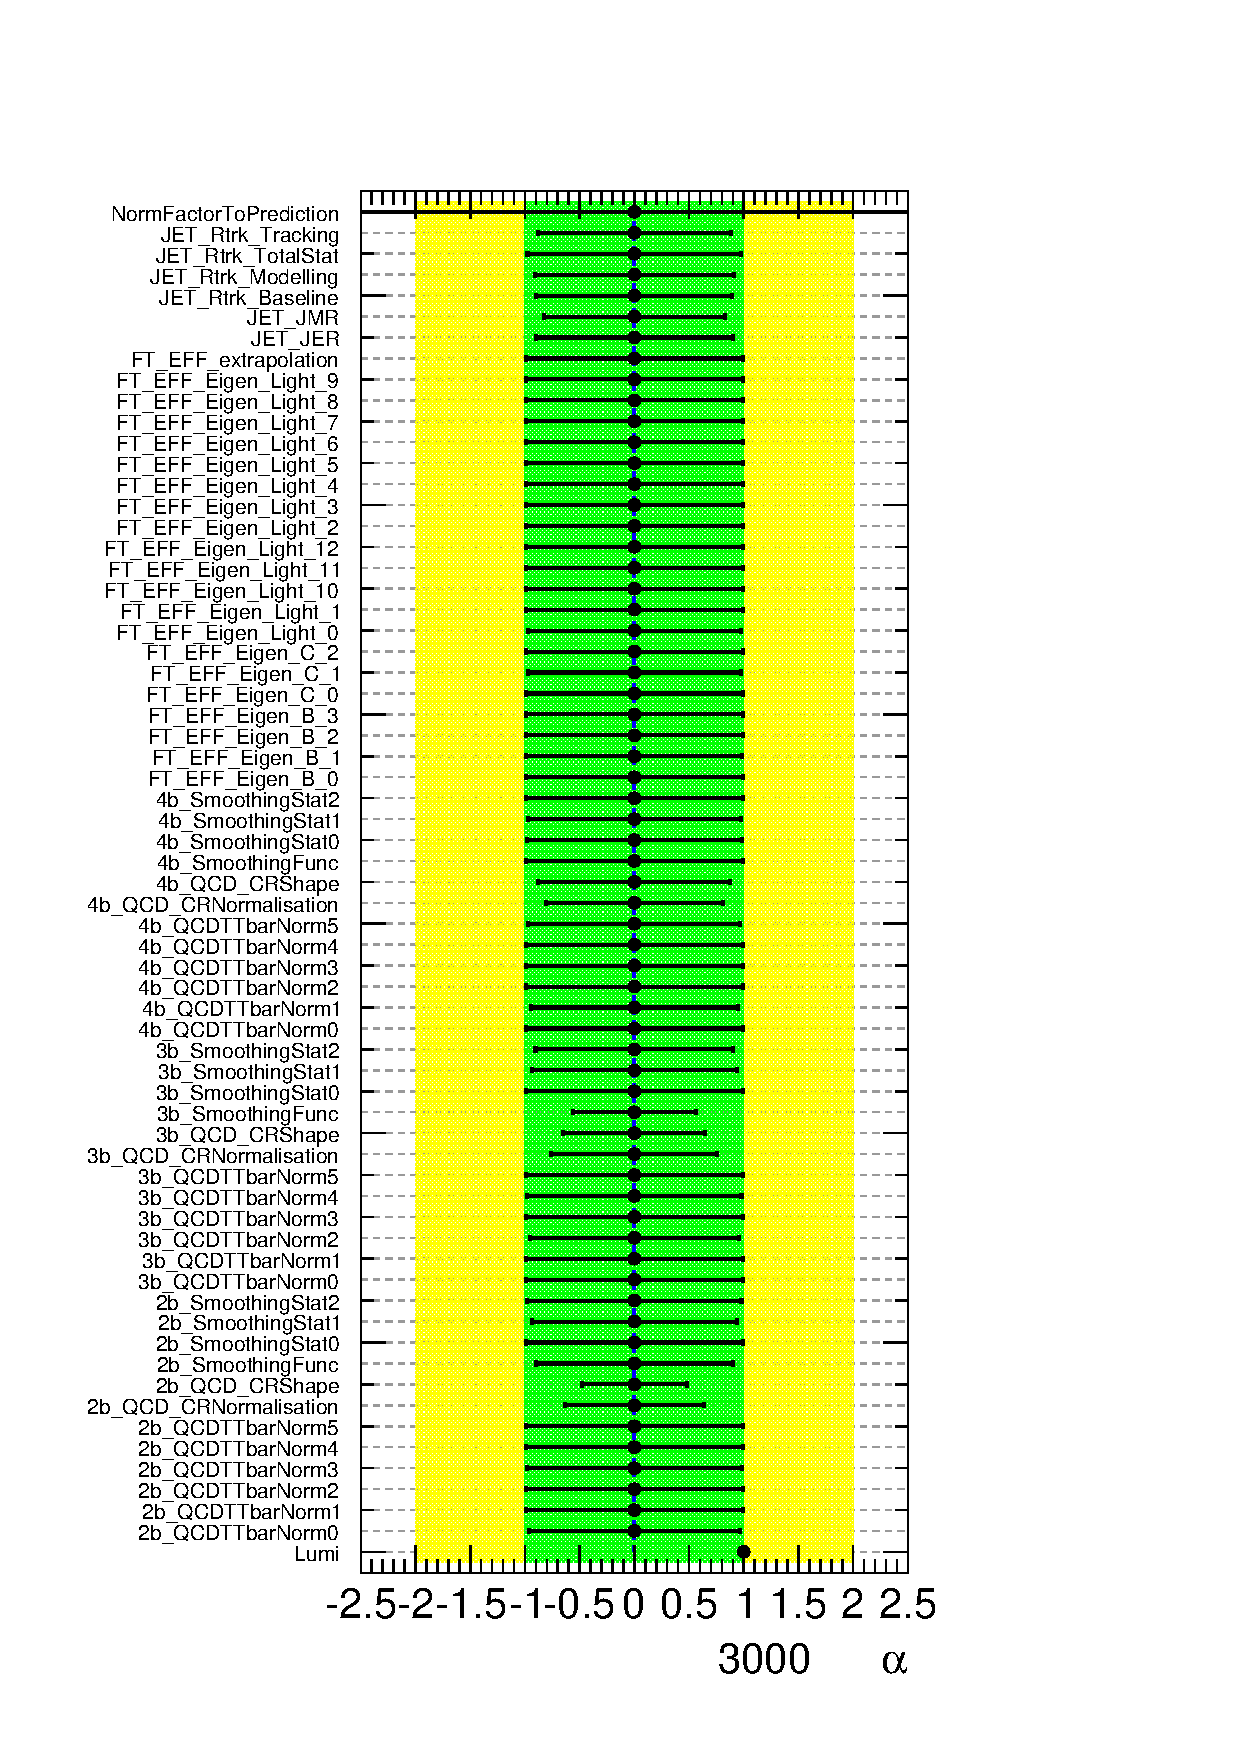
\includegraphics[angle=270, width=0.39\textwidth]{./figures/boosted/app-fitchecks/pulls_3000_asimov.pdf} }
\subfloat[]{ 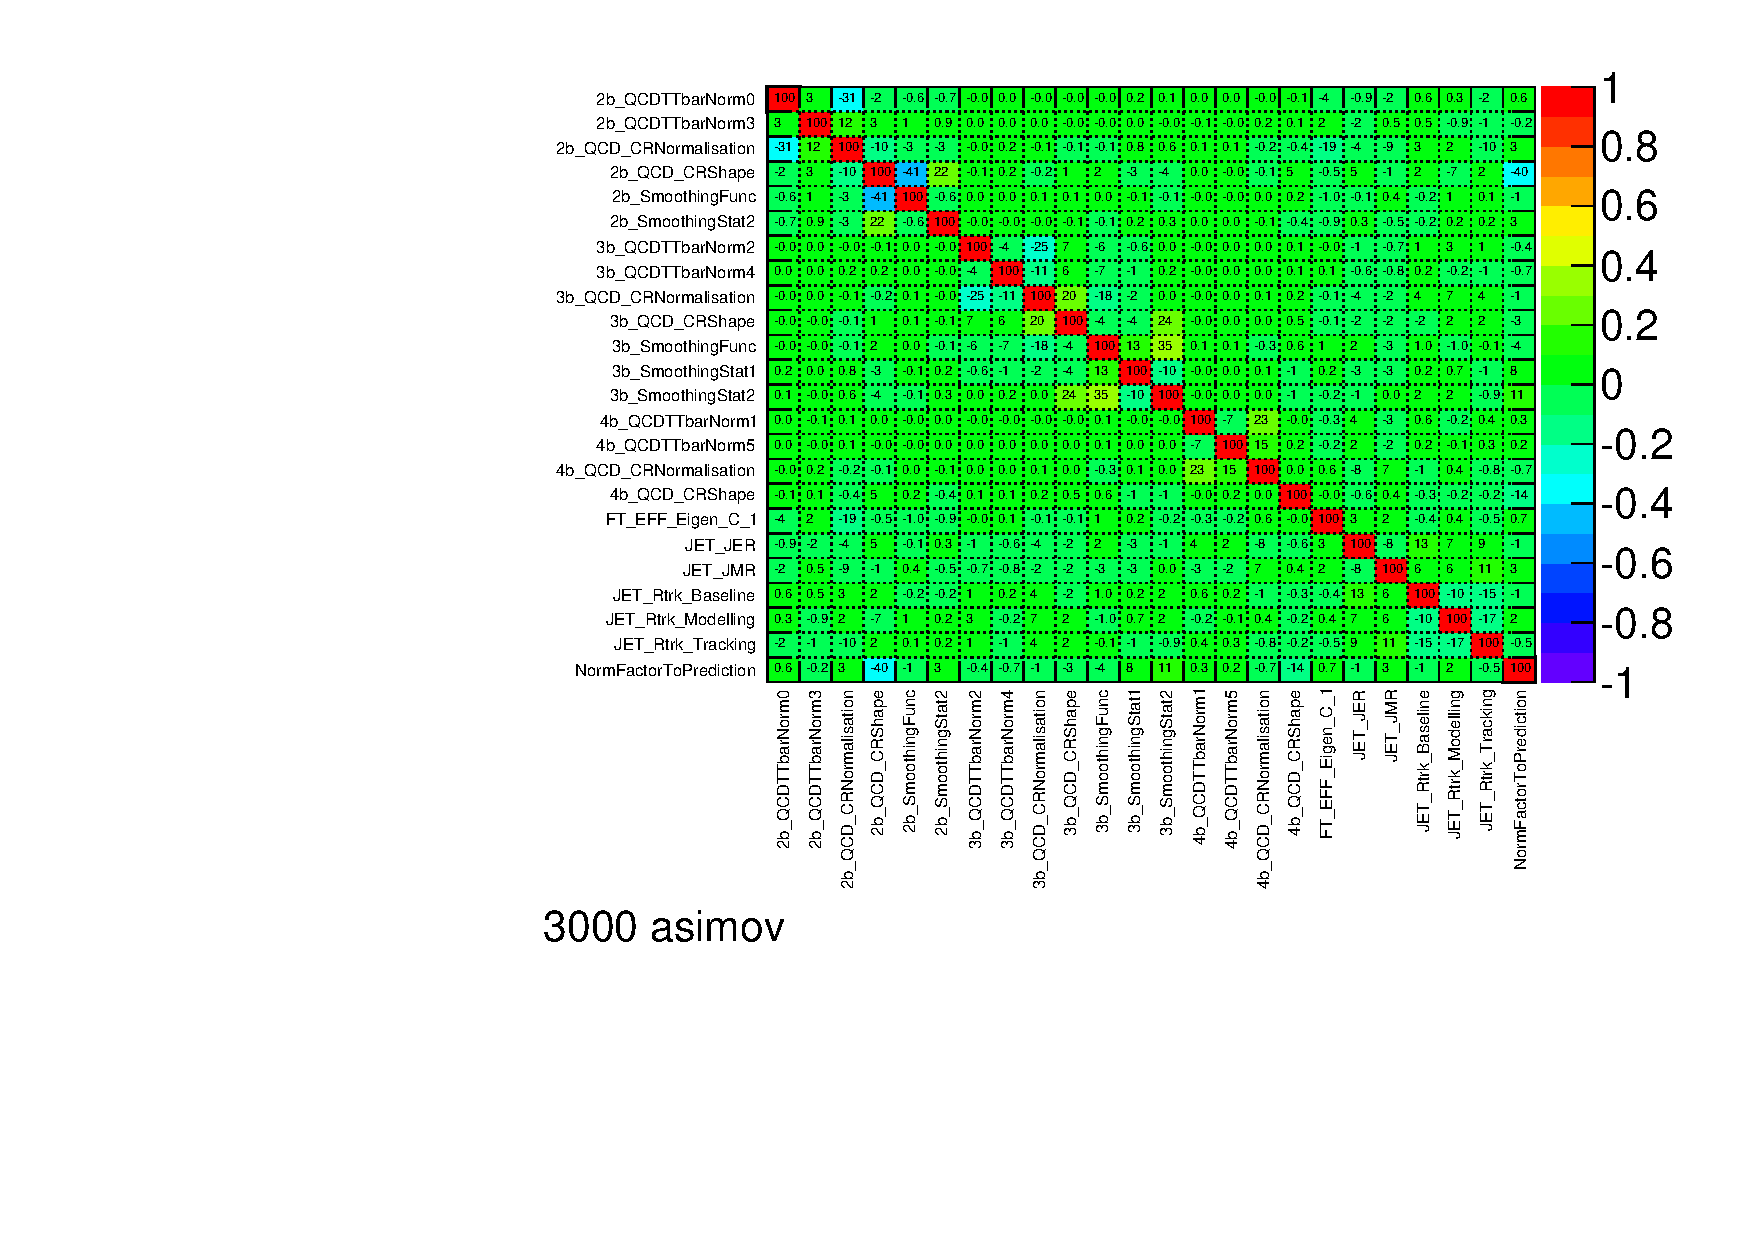
\includegraphics[angle=270, width=0.59\textwidth]{./figures/boosted/app-fitchecks/corr_3000_asimov.pdf} }
\caption{Pulls (a) and correlations (b) for the 3000 GeV mass point.}
\label{fig:fitchecks:pullcorr3000}
\end{center}
\end{figure*}

\begin{figure*}[htbp!]
\begin{center}
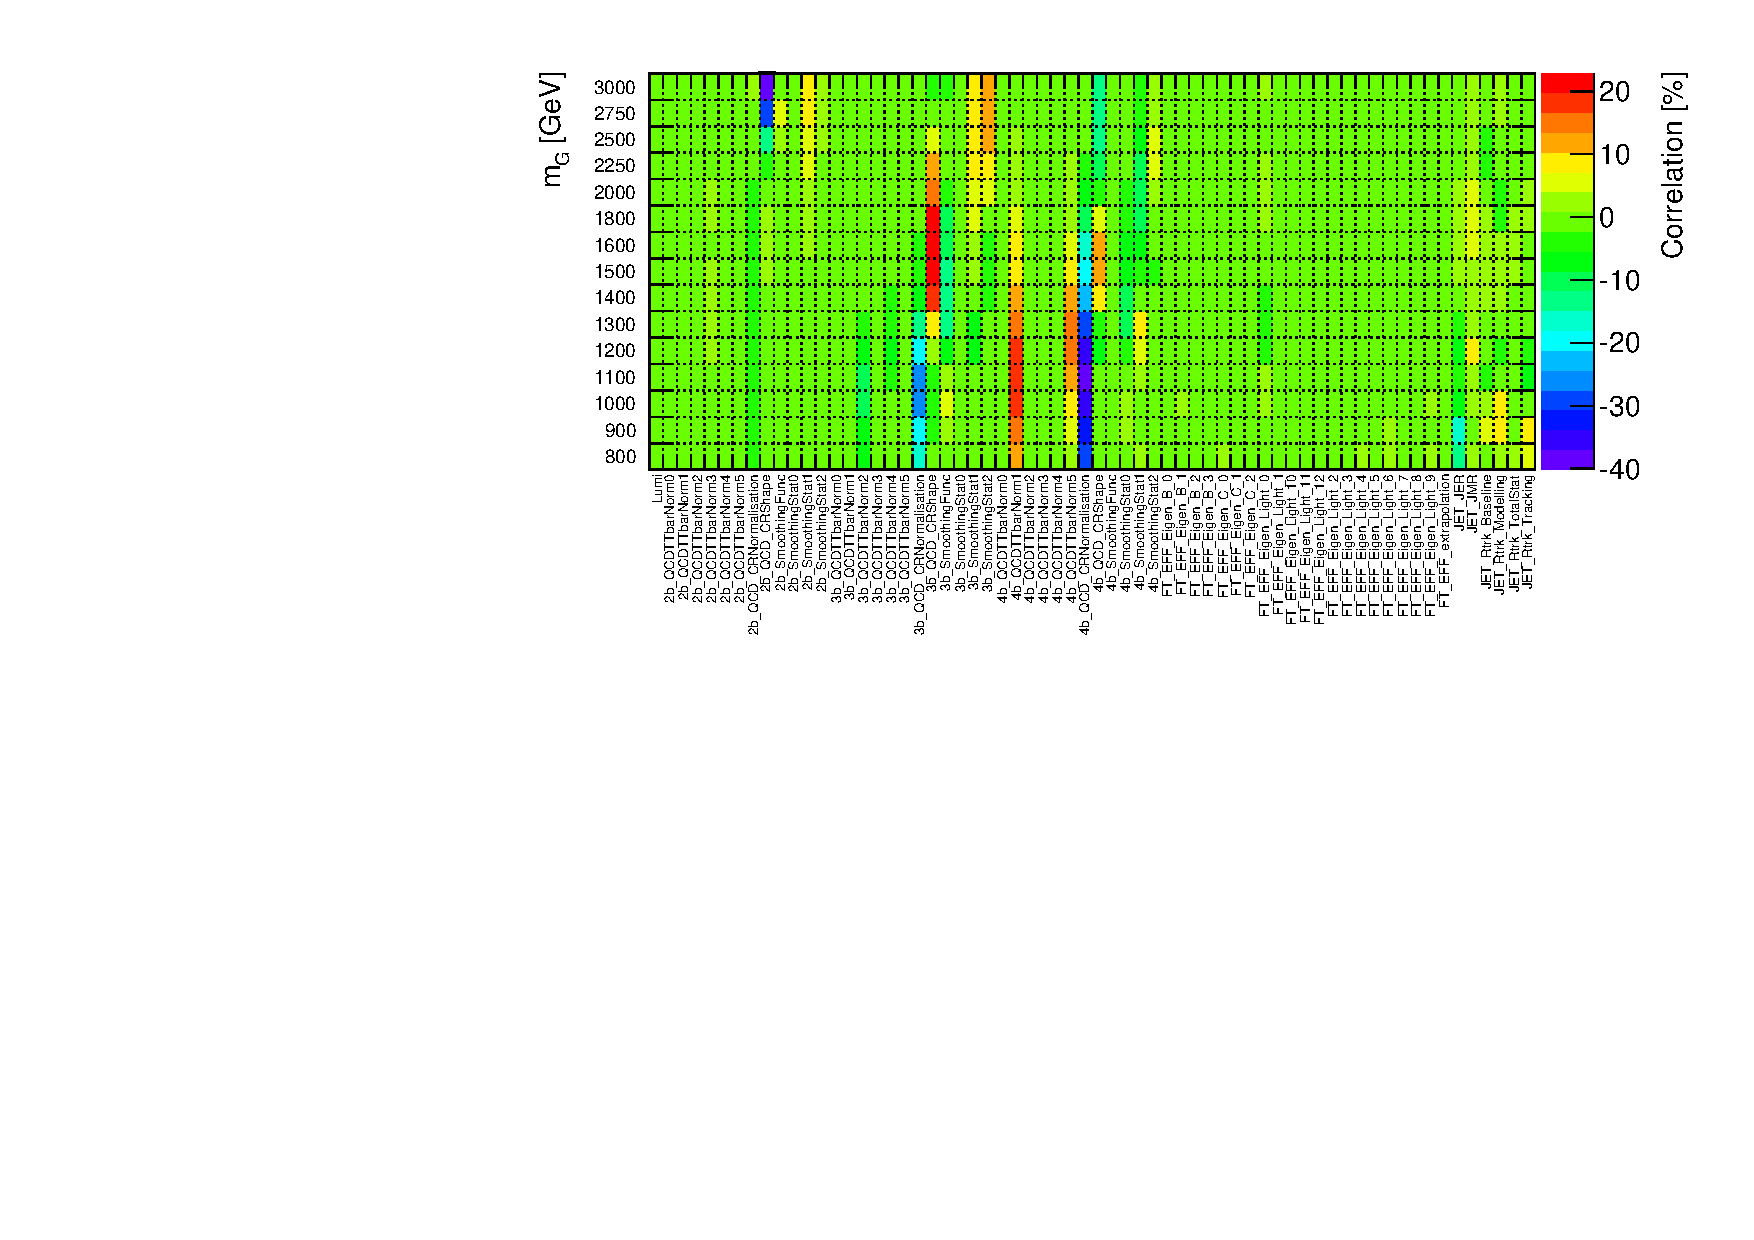
\includegraphics[angle=270, width=0.99\textwidth]{./figures/boosted/app-fitchecks/corr_signal_NPs.pdf}
\caption{The correlation of the signal strength with the nuisance parameters (x-axis) for all mass points (y-axis).}
\label{fig:fitchecks:signalcorr}
\end{center}
\end{figure*}
